% Self-contained Overleaf source. Select pdfLaTeX and compile twice.
\documentclass[11pt,a4paper,oneside]{report}
\usepackage[utf8]{inputenc}
\usepackage[T1]{fontenc}
\usepackage{lmodern}
\usepackage[margin=22mm]{geometry}
\usepackage{microtype}
\usepackage{amsmath,amssymb}
\usepackage{booktabs,longtable,tabularx,array}
\usepackage{enumitem}
\usepackage{xcolor}
\usepackage{listings}
\usepackage{tikz}
\usetikzlibrary{arrows.meta,positioning,fit}
\usepackage{hyperref}
\usepackage{xurl}
\hypersetup{colorlinks=true,linkcolor=blue!45!black,urlcolor=blue!55!black,citecolor=blue!45!black,pdftitle={Android NIDS: Complete Project Development Report}}
\usepackage{fancyhdr}
\pagestyle{fancy}\fancyhf{}\fancyhead[L]{\small Android NIDS development record}\fancyfoot[C]{\thepage}
\setlength{\headheight}{14pt}
\setlength{\parindent}{0pt}\setlength{\parskip}{6pt}
\setlist{itemsep=3pt,topsep=4pt}
\setcounter{tocdepth}{2}
\renewcommand{\arraystretch}{1.18}
\setlength{\tabcolsep}{4pt}
\newcolumntype{Y}{>{\raggedright\arraybackslash}X}
\newcommand{\code}[1]{\nolinkurl{#1}}
\newcommand{\pct}[1]{#1\%}
\newcommand{\important}[1]{\begin{quote}\color{blue!45!black}\textbf{#1}\end{quote}}
\lstset{basicstyle=\ttfamily\footnotesize,breaklines=true,columns=fullflexible,keepspaces=true,frame=single,rulecolor=\color{black!20},backgroundcolor=\color{black!2},showstringspaces=false}
\tikzset{box/.style={draw,rounded corners,align=center,fill=blue!5,inner sep=6pt,font=\small},arr/.style={-{Latex[length=2mm]},thick}}
\emergencystretch=3em
\begin{document}
\hypersetup{pageanchor=false}
\begin{titlepage}
\centering\vspace*{17mm}
{\Huge\bfseries Android NIDS\par}\vspace{7mm}
{\LARGE From paper reconstruction to\par an on-device intrusion-detection pipeline\par}\vspace{12mm}
{\Large Complete development and experimental report\par}\vspace{10mm}
\begin{minipage}{0.88\textwidth}
This report explains the problem, network basics, datasets, preprocessing, model architectures, experiments, actual phone tests, failures, repairs, reproducibility checks and next steps. It is written for a reader with no prior network-security or machine-learning knowledge.

The main narrative starts with the TSANet paper reconstruction. A historical appendix explains the earlier RC4, v5 and v6 work discussed in the conversation. Completed measurements, illustrative calculations, ongoing training and proposed experiments are identified separately.
\end{minipage}
\vfill
\textbf{Evidence cutoff:} 21 November 2026, 04:18 IST\par
\textbf{Current installed detector:} preserved phone-aligned v2\par
\textbf{App version:} \code{0.12.2-aligned-v2-test}, version code 36\par
\textbf{Repository:} \url{https://github.com/vishwajeet-singh-bhati/Android-nids}\par
\vspace{8mm}
{\small Self-contained source: upload this single \code{.tex} file to Overleaf and select pdfLaTeX. No external figures, data files, bibliography file or shell escape are required.}
\end{titlepage}
\pagenumbering{roman}
\hypersetup{pageanchor=true}
\chapter*{How to read this report}
\addcontentsline{toc}{chapter}{How to read this report}
Read Chapters 1--2 first if the domain is new. Chapters 3--7 follow the model-development sequence. Chapters 8--10 explain the Android system, live tests and newly captured data. Chapters 11--12 explain what can be reproduced, what remains unproven and the planned all-class test setup. Appendices contain exact feature layouts, additional candidate results, older approaches and an evidence index.

Throughout the report, \textbf{measured} means a result saved by an actual experiment; \textbf{illustrative} means an explanatory calculation; \textbf{pending} means the relevant experiment has not produced a final accepted result. A software self-check is never counted as a detected attack. A dataset label is not automatically proof that an attack successfully compromised a device.

\important{The most important finding is that high offline benchmark accuracy did not automatically transfer to the phone. The current v2 detected controlled scans, but missed verified HTTP password guessing, SQL injection and XSS examples. The new phone-data experiment addresses this gap; its final results were unavailable at the report cutoff.}

Numbers in percentage tables are percentages unless stated otherwise. A change from 90\% to 95\% is 5 \emph{percentage points}, abbreviated pp. A row, flow segment, endpoint view, request, attack episode, activity card and notification are different units.
\tableofcontents\clearpage
\pagenumbering{arabic}

\chapter{The problem, explained from the beginning}
\section{What we are building}
NIDS means \emph{network intrusion detection system}. The objective is a local Android network-intrusion monitor. It watches traffic involving the phone, turns observations into numbers, estimates whether the traffic is suspicious, assigns a possible attack family, and gives the user a short explanation. The desired balance is high attack detection with few warnings for ordinary use.

The requested final design has three responsibilities. A lightweight model first answers ``Should this traffic be flagged?'' A larger diagnosis model then estimates the attack family for flagged traffic. A local Llama language model rewrites the recorded evidence into readable guidance. The language model does not decide the initial network classification.

For example, suppose another computer tries many closed ports on the phone. The monitor may observe many short failed connections, repeated SYN packets and reset responses. It can group the related warnings into an activity and tell the user that a possible scan was observed. If the Android socket owner cannot be established, the explanation must say ownership is unknown.

The implemented system monitors and warns. No automatic traffic blocking is implemented in this pipeline. It is a research prototype, with important remaining accuracy and generalization limits.

\section{Network vocabulary}
\begin{longtable}{p{0.20\textwidth}p{0.73\textwidth}}
\toprule Term & Beginner explanation\\\midrule\endhead
Packet & A small unit of network communication. A conversation usually contains many packets.\\
Header & Routing and delivery information, such as addresses, transport protocol, ports and TCP flags.\\
Payload & The bytes carried by a packet, such as part of a request, response or encrypted message.\\
IP address & A network address used to deliver traffic to an endpoint. It is not necessarily a person's identity.\\
Port & A numbered service endpoint. A web server or SSH server listens on a port.\\
TCP & A transport protocol that establishes connections and acknowledges delivery.\\
UDP & A transport protocol that sends datagrams without TCP's connection handshake.\\
SYN / ACK / FIN / RST & TCP flags involved in starting, acknowledging, closing or resetting a connection. A SYN by itself is normal and is not proof of a scan.\\
Flow & Packets grouped into a connection-like conversation using protocol and both address/port pairs. Our online system may split a long conversation into several segments.\\
Context & Information about recent completed connections, so a flow is interpreted alongside nearby activity.\\
Feature & One numeric measurement supplied to a model, such as a packet count or duration.\\
Label & The reference answer associated with training/evaluation data. Labels come from dataset metadata or independently verified test actions, not model predictions.\\
Model / parameters & A mathematical function and the learned numerical weights inside it.\\
Logit & An unrestricted model score before converting it to a probability-like value.\\
Sigmoid / softmax & Functions converting one logit into a binary score, or seven logits into seven relative scores. These scores are not guarantees of correctness.\\
Epoch / batch / seed & A training cycle; a group of examples used for one update; and a random-generator setting used for repeatability. Some older sampling epochs are not full passes over a corpus.\\
Checkpoint & Saved model weights and often optimizer/random state, allowing evaluation or training resume.\\
\bottomrule
\end{longtable}

\section{Which network layers are used?}
The phone capture starts from link-layer frames or Android's cooked capture framing. The parser reads IP-level information, then TCP/UDP transport information. It measures timing, direction, payload lengths and flags. For supported cleartext traffic, it also extracts a few application-level indicators from bounded payload/header prefixes.

The current numeric classifier therefore mainly uses \textbf{network/transport traffic statistics with limited application-protocol evidence}. It is not fed an entire raw packet as text. It does not receive a complete website, full request body, application source code, Android permissions or arbitrary phone files as its input.

HTTPS and SSH application contents remain encrypted. The system can still observe available connection characteristics, but cannot directly read an encrypted password or SQL payload. The current feature pipeline handles TCP/UDP; a network attack carried only by other protocols cannot be assumed to have direct model coverage merely because a broad output category has a similar name.

Literal addresses and port numbers are used to group packets, build histories and attach evidence. They are not literal identity inputs to the current classifiers. Llama receives selected structured evidence after detection, not the entire captured packet stream.

\section{The seven labels and their meanings}
\begin{longtable}{p{0.18\textwidth}p{0.75\textwidth}}
\toprule Label & Meaning in this project\\\midrule\endhead
Benign & A reference label for normal traffic within the stated dataset or controlled experiment. It does not certify that all activity from an application is harmless.\\
Bot & The dataset's bot-activity category. Harmless periodic connections can resemble some communication patterns, so periodicity alone does not prove bot infection.\\
Brute Force & In the seven-family CIC-IDS2017 mapping, FTP-Patator and SSH-Patator. HTTP login guessing belongs to Web Attack here.\\
DDoS & The dataset's distributed-denial-of-service label. Our earlier single-PC HTTP burst did not establish distributed service disruption.\\
DoS & Four dataset variants: GoldenEye, Hulk, Slowhttptest and slowloris. Each has its own traffic characteristics.\\
Port Scan & Probing multiple service ports. Expected discovery or diagnostics require matching normal controls.\\
Web Attack & HTTP brute-force/login guessing, XSS and SQL injection. Broad-family results do not establish equal coverage of all three subtypes.\\
\bottomrule
\end{longtable}
\code{Unclassified} is an output-policy fallback for a flagged event without reliable attack typing. It is not an eighth learned class.

\section{Training, validation, test and inference}
During training, the classifier receives feature values and a separate known label. A loss function measures the prediction error, and an optimizer adjusts the learned weights. The label is used to compute loss; it is not inserted into the feature vector as an answer hint. Repeating this process across batches/epochs produces a checkpoint.

Validation data is used to choose settings, checkpoints or thresholds without gradient updates on those examples. A reserved test is used for final evaluation after choices are frozen. Once test results have influenced a repair decision, that test has become opened development evidence; it cannot be presented as newly blind on a later attempt. Independent sessions/campaigns matter because many rows can describe one underlying event.

Inference means running a fixed model on new input. The tested phone does not continuously retrain these classifier weights. Its recent-connection history does update as packets arrive, but changing a history buffer is not changing learned weights. Evaluation uses inference mode: training-time dropout is disabled and BatchNorm uses its stored training statistics.

The word \emph{context} also has two separate meanings here. Connection context is the numeric history used by the detector. Llama prompt context is the text used to write one explanation. Caching Llama weights does not merge those histories or make the language model learn from every phone request.

\section{How we judge performance}
An attack flagged is a true positive (TP); an attack missed is a false negative (FN). Normal traffic flagged is a false positive (FP); normal traffic left quiet is a true negative (TN).
\begin{align*}
\text{Precision}&=\frac{TP}{TP+FP}, & \text{Recall}&=\frac{TP}{TP+FN},\\
F_1&=\frac{2TP}{2TP+FP+FN}, & \text{Benign FPR}&=\frac{FP}{FP+TN}.
\end{align*}
Precision asks whether warnings are usually correct. Recall asks whether attacks are usually detected. Macro F1 averages each class equally; weighted F1 gives larger classes more influence. If 99 of 100 examples are normal, a model predicting ``normal'' for everything achieves 99\% accuracy while detecting no attacks. This is why headline accuracy is insufficient.

\textbf{Binary detection and exact typing differ.} A Web Attack flagged as Unclassified is detected but not correctly typed. A confident wrong label is still wrong. A single attack episode can generate hundreds of flow flags, which may be grouped into a few notifications. Those counts cannot be converted directly into attack accuracy.

\chapter{Development map and datasets}
\section{The sequence of work}
\begin{longtable}{p{0.12\textwidth}p{0.34\textwidth}p{0.47\textwidth}}
\toprule Stage & Built or investigated & Why the next step was needed\\\midrule\endhead
Earlier work & AndMal-based packet windows; RC4; v5 general/specialist/distillation; v6 cascade. & False-positive, coverage and end-to-end gating problems remained. Historical appendix retains their limits.\\
Paper & Reconstructed TSANet, then independent 30\% and 40\% pruning branches. & Bot/Web recall and benign false positives were weak despite roughly 97\% accuracy.\\
Context & Added 78 causal history features and an equal-capacity zero-context control. & Offline results improved sharply; dependence/visibility and real-device validity needed investigation.\\
Initial Android & Exported the context model, added local explanations, history, attribution and background monitoring; ran bounded traffic probes. & Technical operation worked, but the probes produced no flags. Matching tensor size did not ensure matching feature meaning.\\
Aligned v2 & Rebuilt inputs from raw PCAP with shared Kotlin code; trained a small gate and larger diagnosis. & Offline results were strong overall but Bot precision failed; a controlled repair was investigated.\\
Repair v3 & Compared loss/sampling changes, calibration and joint routing. & Fewer benign flags came with unacceptable Bot/Web regressions; preserved v2 remained the fallback.\\
V2 phone tests & Installed fixed v2 and verified real controlled target effects. & Scans worked; verified Web examples and bounded resource denial were missed.\\
New phone data & Built DatasetLab, captured 20 quality-gated sessions and launched six training jobs. & Final candidate comparison and native/live validation remain pending at the cutoff.\\
Submission & Published current source, reproducibility guides and tested CI. Discussed extending coverage using extra local PCs over SSH. & Multi-source DDoS, real FTP/SSH targets and a working bot-like controller are still preparation tasks.\\
\bottomrule
\end{longtable}

\section{Datasets: similar names do not mean identical tasks}
\textbf{CIC-IDS2017} provides labeled laboratory network traffic across five weekdays, as both flow CSVs and raw captures. The CSV experiment uses completed-flow statistics. The phone-aligned experiment re-extracts different, phone-visible flow segments from the raw captures. They are distinct cohorts with distinct input semantics, even though their publisher and broad label names agree. Publisher: \url{https://www.unb.ca/cic/datasets/ids-2017.html}.

\textbf{AndMal2017 in the earliest project} concerned traffic associated with benign and Android malware applications. The locally recorded inventory contains 2,126 captures: 1,700 Benign, 104 Adware, 112 Scareware, 109 SMSMalware and 101 Ransomware. Its processed corpus had 827,225 windows: 659,570 benign and 167,655 malicious-associated, from 648,462 unique flows. A window had 32 packets, 12 metadata channels and up to 128 payload bytes per packet. A cap of 400 examples/capture and 1,000,000 records/capture applied in that earlier preprocessing. A malicious-app-associated capture label is not proof that every packet is an attack.

\textbf{CIC-AAGM2017} is a separate local corpus of 242 captures: 173 Benign, 62 Adware and 7 General Malware. The aligned experiment uses only its \emph{publisher-benign subset} as Android controls. It does not label the entire malware collection benign. Complete-file integrity checks accepted 172 of the 173 benign captures. Publisher: \url{https://www.unb.ca/cic/datasets/android-adware.html}.

\textbf{PARROT2025} supplied 320 local captures, four traces for each of 80 ordinary apps, from an Android emulator/interception environment. Complete-file checks accepted 319 captures. These are useful Android negative controls, but not certified clean Pixel everyday traffic. Recorded publisher provenance: \url{https://zenodo.org/records/16368932}.

\textbf{New Pixel data} contains actual controlled requests and target effects from our owned phone and disposable app. It supplements the original corpus rather than replacing it. Normal background flows remain unlabeled unless independently identified as a controlled action. No new Bot, FTP/SSH, DoS or DDoS positive labels were added by this collection.

CICMalDroid2020, UNSW-NB15 and NSL-KDD were proposals found in local records, not datasets demonstrated as used to train the current paper/context/aligned models. The report does not silently count them as training evidence.

\section{Original paper/context class counts}

{\small
\begin{longtable}{@{}lrrr@{}}
\toprule
Class & Train & Test & Retained total\\\midrule\endhead
Benign & 1,589,924 & 681,396 & 2,271,320\\
Bot & 1,369 & 587 & 1,956\\
Brute Force & 9,682 & 4,150 & 13,832\\
DDoS & 89,618 & 38,407 & 128,025\\
DoS & 176,198 & 75,514 & 251,712\\
Port Scan & 111,163 & 47,641 & 158,804\\
Web Attack & 1,526 & 654 & 2,180\\
\bottomrule\end{longtable}
}

The imbalance comes from the observed corpus. Millions of rows overall do not imply abundant independent Bot or Web episodes. Duplicates, endpoint views and segments can increase row counts without adding independent attack situations.

\textbf{Version names require context.} The earlier two-detector network release called RC4 and the later app \code{0.11.3-context-rc4} are different designs. The latter is the 110-input TSANet-context deployment. Neither name denotes the current 147-input v2 cascade. Likewise, ``repair v3'' is a controlled experiment on v2, not a deployed replacement.

\section{Raw-packet aligned class counts}

{\small
\begin{longtable}{@{}lrrr@{}}
\toprule
Class & Train views & Validation views & Test views\\\midrule\endhead
Benign & 4,214,044 & 1,029,548 & 940,095\\
Bot & 3,130 & 652 & 640\\
Brute Force & 11,334 & 2,432 & 2,442\\
DDoS & 82,746 & 17,572 & 17,840\\
DoS & 422,234 & 90,672 & 90,084\\
Port Scan & 222,584 & 47,698 & 47,688\\
Web Attack & 602 & 150 & 140\\
\bottomrule\end{longtable}
}

The aligned splits contain 4,956,674 training, 1,188,724 validation and 1,098,929 test views. A view represents what a selected endpoint could observe; an underlying connection can generate multiple segments and endpoint views. Connection groups are kept together. The split is approximately 70/15/15 at the grouping level, with seeds 8621/8622; exact row percentages differ across corpora/groups.


{\small
\begin{longtable}{@{}lrrr@{}}
\toprule
Aligned source & Train views & Validation views & Test views\\\midrule\endhead
Monday & 713,820 & 153,850 & 155,724\\
Tuesday & 623,354 & 132,568 & 133,200\\
Wednesday & 1,049,200 & 226,314 & 226,438\\
Thursday & 706,312 & 153,084 & 150,310\\
Friday & 885,196 & 191,972 & 193,902\\
PARROT & 406,030 & 242,396 & 132,945\\
AAGM & 572,762 & 88,540 & 106,410\\
\bottomrule\end{longtable}
}



{\small
\begin{longtable}{@{}lrrr@{}}
\toprule
Selected fine label & Train & Validation & Test\\\midrule\endhead
FTP-Patator & 7,196 & 1,550 & 1,562\\
SSH-Patator & 4,138 & 882 & 880\\
DoS GoldenEye & 13,466 & 2,822 & 2,862\\
DoS Hulk & 377,988 & 81,272 & 80,722\\
DoS Slowhttptest & 16,260 & 3,516 & 3,484\\
DoS slowloris & 14,520 & 3,062 & 3,016\\
Web Attack Brute Force & 454 & 104 & 104\\
Web Attack XSS & 136 & 42 & 34\\
Web Attack Sql Injection & 12 & 4 & 2\\
\bottomrule\end{longtable}
}

Only 12 SQL training views and two SQL test views existed in the raw aligned corpus. A broad Web score therefore cannot support a strong SQL-injection reliability claim. These counts, rather than overall dataset size, motivated collecting verified phone examples.

\chapter{Stage 1: reconstructing the TSANet paper}
\section{What the paper supplied and what was missing}
The supplied six-page paper was \emph{A Lightweight Embedded Intelligent Threat Detection System Using TSANet on Android Platforms}, Malode et al., ISED 2025, DOI \href{https://doi.org/10.1109/ISED67359.2025.11404952}{10.1109/ISED67359.2025.11404952}. Its architecture uses spatial and temporal attention on 32 flow features. It states Adam, learning rate 0.001, batch size 256, ten initial epochs and five pruning fine-tuning epochs.

The authors' code, exact feature list/order, train/test memberships and several implementation details were unavailable. The user chose \textbf{70\% training / 30\% testing}. We recorded assumptions before training and reported our measured figures rather than altering training until a desired paper number appeared.
\begin{longtable}{p{0.30\textwidth}p{0.63\textwidth}}
\toprule Unspecified detail & Declared reconstruction\\\midrule\endhead
Exact split & Stratified random 70/30, seed 42, saved row IDs and indices. No hidden validation subtraction from the 70\% training set.\\
32 features/order & Fixed numeric flow-feature list in Appendix A; selected before test inference.\\
Cleaning/scaling & Header/label normalization; exclude out-of-scope labels; drop nonfinite selected values; retain duplicates; training-only StandardScaler.\\
Convolution kernel/padding & Kernel 3, padding 1 in the spatial branch; kernel 1 attention gate.\\
Attention nonlinearities & Sigmoid spatial gate; softmax over feature positions for temporal attention.\\
Dense width and normalization & Hidden Dense 64/ReLU; BatchNorm epsilon 0.001 and momentum 0.01.\\
Initialization & PyTorch defaults, fixed seed 42, FP32 and recorded deterministic settings.\\
Pruning method & Fixed global magnitude masks over matrix weights, including recurrent matrices; biases and BatchNorm excluded.\\
Fine-tuning continuation & Reset Adam independently for each pruning branch; fixed masks cannot regrow.\\
Metric averaging & Report both macro and weighted precision/recall/F1 because the paper's averaging rule is not disclosed.\\
Mobile imputation/quantization & Not claimed reproduced: exact missing-feature defaults, interpolation/adaptation data and quantization recipe are unavailable.\\
\bottomrule
\end{longtable}

\section{Cleaning and training/test preprocessing}
The archive \code{GeneratedLabelledFlows.zip} contains eight labeled CSV members spanning five weekdays. Normalize header spaces and label replacement characters, map fine labels to the seven families, and ignore recorded blanks. From 2,830,743 labeled rows, exclude 36 Infiltration and 11 Heartbleed rows because they are outside the seven named classes. Drop 2,867 rows with nonfinite/unparseable selected features. Retain 2,827,829 rows: 1,979,480 train and 848,349 test.

For feature $j$, compute training mean $\mu_j$ and scale $\sigma_j$, then use
\[z_j=(x_j-\mu_j)/\sigma_j.\]
Apply the \emph{same fitted values} to test rows. Test preprocessing never learns a new mean or scale. No class balancing or resampling was used in this reconstruction; training used natural class frequencies and unweighted cross-entropy.

\section{Exact architecture and shapes}
\begin{center}
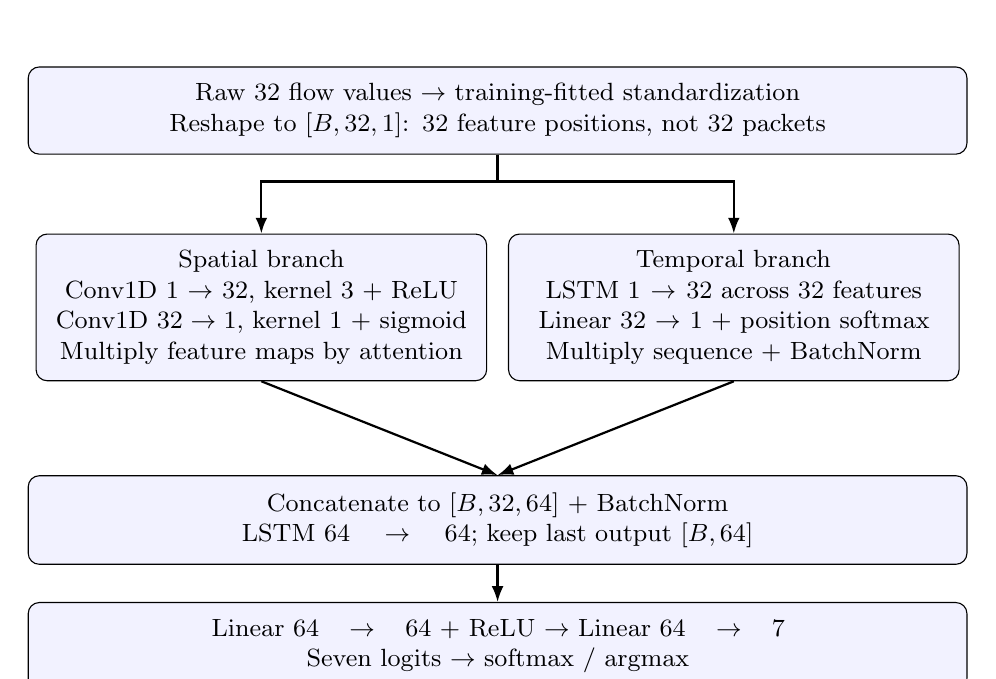
\begin{tikzpicture}[node distance=7mm and 8mm]
\node[box,text width=11.5cm] (input) at (0,0) {Raw 32 flow values $\rightarrow$ training-fitted standardization\\Reshape to $[B,32,1]$: 32 feature positions, not 32 packets};
\node[box,text width=5.3cm] (sp) at (-3,-2.5) {Spatial branch\\Conv1D $1\to32$, kernel 3 + ReLU\\Conv1D $32\to1$, kernel 1 + sigmoid\\Multiply feature maps by attention};
\node[box,text width=5.3cm] (tm) at (3,-2.5) {Temporal branch\\LSTM $1\to32$ across 32 features\\Linear $32\to1$ + position softmax\\Multiply sequence + BatchNorm};
\node[box,text width=11.5cm] (f) at (0,-5.2) {Concatenate to $[B,32,64]$ + BatchNorm\\LSTM $64\to64$; keep last output $[B,64]$};
\node[box,text width=11.5cm] (out) at (0,-6.8) {Linear $64\to64$ + ReLU $\rightarrow$ Linear $64\to7$\\Seven logits $\rightarrow$ softmax / argmax};
\draw[arr] (input.south) -- (0,-0.9) -| (sp.north);
\draw[arr] (input.south) -- (0,-0.9) -| (tm.north);
\draw[arr] (sp.south) -- (f.north);\draw[arr] (tm.south) -- (f.north);\draw[arr] (f.south) -- (out.north);
\end{tikzpicture}
\end{center}
There are \textbf{42,761 trainable parameters}; $B$ denotes batch size in the diagram. Here ``temporal'' refers to the recurrent branch traversing a fixed ordered feature sequence. The paper reconstruction is not a packet-by-packet network-language model.

Seven logits become probabilities $p_k=\exp(l_k)/\sum_i\exp(l_i)$. The predicted class is the largest logit. A non-Benign argmax is counted as an attack prediction. This stage has no separately calibrated binary gate.

\section{Training and pruning}
Train the baseline for ten full epochs with Adam, learning rate 0.001 and batch 256. No early stopping is used. Save every epoch, last and best-training-loss checkpoints, but use the \emph{fixed final epoch} for the declared paper comparison.

Start both pruning branches from baseline epoch 10. Mask the smallest absolute matrix weights globally: 12,508 of 41,696 eligible weights at 30\%, or 16,678 at 40\%. Fine-tune each for five epochs, masking gradients and re-zeroing weights after updates. Both branches preserve the 42,761-parameter dense architecture. Zeros alone do not guarantee a smaller dense file or faster Android execution.

\section{Results and comparison with the paper}

{\small
\begin{longtable}{@{}lrrrrr@{}}
\toprule
Variant & Accuracy & Macro F1 & Attack recall & Benign FPR & Benign FP\\\midrule\endhead
Baseline & 97.0256 & 76.6327 & 91.7953 & 1.68933 & 11,511\\
Pruned 30\% & 97.3240 & 77.1588 & 95.2472 & 2.16379 & 14,744\\
Pruned 40\% & 97.3340 & 76.2494 & 95.1364 & 2.12343 & 14,469\\
\bottomrule\end{longtable}
}

The paper's baseline \emph{test} accuracy is 97.35\%; 98.0\% is its reported baseline \emph{training} accuracy. The stated 30\%-pruned test accuracy is 98.30\%. The precise 40\% point is not stated numerically. Our baseline differed by approximately $-0.32$ pp and our 30\% variant by $-0.98$ pp. Undisclosed split/feature/implementation details prevent exact causal attribution of these gaps. The paper's limited-mobile-feature 93.2\% result and Android timing were not claimed reproduced.

The paper reports precision/recall/F1 of 98.6/97.9/98.1\% without a disclosed averaging rule. Our reproducible averages are shown separately rather than selecting whichever average looks closer:

{\small
\begin{longtable}{@{}lrr@{}}
\toprule
Variant & Macro $P/R/F_1$ & Weighted $P/R/F_1$\\\midrule\endhead
Baseline & 95.121 / 72.036 / 76.633 & 97.024 / 97.026 / 96.980\\
Pruned 30\% & 95.928 / 73.292 / 77.159 & 97.426 / 97.324 / 97.313\\
Pruned 40\% & 96.196 / 72.752 / 76.249 & 97.432 / 97.334 / 97.318\\
\bottomrule\end{longtable}
}



{\small
\begin{longtable}{@{}lrrr@{}}
\toprule
Class & Baseline $P/R/F_1$ & Pruned 30\% $P/R/F_1$ & Pruned 40\% $P/R/F_1$\\\midrule\endhead
Benign & 98.00 / 98.31 / 98.15 & 98.82 / 97.84 / 98.33 & 98.80 / 97.88 / 98.33\\
Bot & 99.12 / 38.50 / 55.46 & 97.01 / 38.67 / 55.30 & 96.64 / 39.18 / 55.76\\
Brute Force & 97.64 / 77.90 / 86.66 & 99.57 / 78.43 / 87.75 & 99.63 / 78.14 / 87.59\\
DDoS & 99.91 / 98.57 / 99.24 & 99.71 / 99.55 / 99.63 & 99.87 / 99.54 / 99.70\\
DoS & 91.03 / 88.77 / 89.89 & 88.20 / 95.05 / 91.50 & 88.40 / 94.86 / 91.52\\
Port Scan & 90.31 / 94.09 / 92.16 & 90.03 / 95.39 / 92.63 & 90.04 / 95.38 / 92.63\\
Web Attack & 89.83 / 8.10 / 14.87 & 98.15 / 8.10 / 14.97 & 100.00 / 4.28 / 8.21\\
\bottomrule\end{longtable}
}

The 30\%-pruned model's Web recall was 8.10\% and Bot recall 38.67\%, with 14,744 benign rows flagged. Accuracy near 97\% hid these class failures. The 40\% variant's slightly higher accuracy did not make it uniformly better: its macro F1 was lower.

\section{Executed input-to-output walkthrough}
The following values come from actual CPU execution of the frozen exports for this report. The sample-selection rule is the first test row of each selected class in the \emph{already-opened historical cohort}; it is not a new accuracy experiment or a model-selection step. Only a few feature values are reproduced, not a dataset or complete packet record.

For the first Benign example, the first five raw values are $[60{,}921,1,1,40,94]$: duration in microseconds, forward/backward packets, and forward/backward payload bytes. Duration is standardized using mean $14{,}810{,}440$ and scale $33{,}679{,}380$:
\[(60{,}921-14{,}810{,}440)/33{,}679{,}380=-0.437939.\]
The other 31 coordinates are standardized with their own stored statistics. The network processes the resulting tensor and predicts Benign.

A more informative first Web-labeled example has first five values $[5{,}722{,}059,3,1,0,0]$. Its duration becomes approximately $-0.269850$. The baseline gives Benign about 0.826422 and Web Attack 0.171095, so it predicts Benign and misses this labeled example. The 30\%-pruned model likewise predicts Benign, about 0.788683 versus 0.209713 Web. Pruning did not supply missing behavioral context.

\chapter{Stage 2: adding context across connections}
\section{The reason for the change}
A single short connection may look the same when caused by a normal application or an attacker. The original diagnostics found 207 of 360 missed Bot rows and 2,146 of 2,176 missed scan rows equal to a Benign training vector across all 32 input features. This demonstrates numeric input ambiguity; it does not by itself prove that the publisher labels were wrong.

We added information about nearby completed connections: how many occurred, how many peers/ports appeared and what response patterns were seen. A single failed connection can be ordinary; many related failures can provide additional evidence.

\section{The 78 context features}
For each of the source and destination roles, compute 13 aggregates over 120, 300 and 900 seconds. Eight values are log-transformed counts: flows, outgoing/incoming packets and bytes, distinct peers, remote ports and local ports. Five are fractions: no peer-direction packets, reset present, SYN present, TCP and UDP.
\[3\text{ windows}\times2\text{ roles}\times13\text{ statistics}=78.\]
The full input is $32+78=110$ values. A flow occurrence count of 48 becomes $\log(1+48)=3.891820$; it is not passed as the literal count 48 in that context coordinate.

Only training rows populate the unlabeled history bank, for both training and test queries. Include definitely prior, completed observations in the relevant window; exclude self, future, tied and uncertain timing. CSV timestamps have second/minute precision and ambiguous hours, so interval-safe rules and the observed daytime schedule are used. Labels, model predictions, literal endpoint identities and absolute times are excluded from the model tensor. Context scaling fits training rows only.

\section{Architecture and fair comparison}
The original TSANet produces a 64-value representation. A new context branch is Linear $78\to32$, ReLU, Linear $32\to16$, ReLU. Concatenate the 64 flow values and 16 context values; apply Linear $80\to64$, ReLU, Linear $64\to7$. The full model has \textbf{46,841 parameters}.

An equal-capacity control has the same architecture and initialization but receives zeros for context \emph{after normalization}. This separates the contribution of information from the contribution of extra parameters. Both arms preserve the original rows/order, 32 flow inputs, split, seed, optimizer, loss, batch size and ten-plus-five epoch budget. Both have independent 30\% pruning branches. No extra data or test-selected checkpoint is introduced in this comparison.


{\small
\begin{longtable}{@{}lrrrr@{}}
\toprule
Same-size arm & Accuracy & Macro F1 & Attack recall & Benign FPR\\\midrule\endhead
Control, unpruned & 97.1808 & 76.9501 & 91.9570 & 1.53420\\
Context, unpruned & 99.9815 & 98.1405 & 99.9311 & 0.00484\\
Control, pruned 30\% & 97.2454 & 76.1135 & 95.1855 & 2.24612\\
Context, pruned 30\% & 99.9850 & 98.6028 & 99.9491 & 0.00558\\
\bottomrule\end{longtable}
}


{\small
\begin{longtable}{@{}lrrr@{}}
\toprule
Class & Original pruned $P/R/F_1$ & Same-size control $P/R/F_1$ & With context $P/R/F_1$\\\midrule\endhead
Benign & 98.82 / 97.84 / 98.33 & 98.81 / 97.75 / 98.28 & 99.99 / 99.99 / 99.99\\
Bot & 97.01 / 38.67 / 55.30 & 99.56 / 38.67 / 55.71 & 95.82 / 85.86 / 90.57\\
Brute Force & 99.57 / 78.43 / 87.75 & 99.51 / 78.19 / 87.57 & 100.00 / 99.98 / 99.99\\
DDoS & 99.71 / 99.55 / 99.63 & 99.51 / 99.60 / 99.55 & 99.99 / 99.99 / 99.99\\
DoS & 88.20 / 95.05 / 91.50 & 87.62 / 95.11 / 91.21 & 99.99 / 100.00 / 99.99\\
Port Scan & 90.03 / 95.39 / 92.63 & 90.10 / 95.12 / 92.54 & 99.99 / 100.00 / 99.99\\
Web Attack & 98.15 / 8.10 / 14.97 & 100.00 / 4.13 / 7.93 & 99.54 / 99.85 / 99.69\\
\bottomrule\end{longtable}
}

Compared with the original pruned reconstruction, context-pruned accuracy increased from 97.3240\% to 99.9850\%, macro F1 from 77.1588\% to 98.6028\%, and benign flags fell from 14,744 to 38 on the same 848,349 test rows. Compared with its equal-capacity pruned control, the gain was 2.7397 pp accuracy and 22.4894 pp macro F1. Bot remained weaker than other classes at 85.86\% recall.

\section{Executed dry run with and without context}
For the same first Web-labeled historical row described in Chapter 3, the first eight context coordinates are approximately
\[[3.891820,5.690360,5.043425,10.793352,12.119926,0.693147,0.693147,3.526361].\]
These summarize the source role in the first 120-second window. The first value corresponds to 48 prior eligible flow occurrences. Distinct peer and remote-port values of $\log 2$ each correspond to one distinct peer and one distinct remote port.

The zero-context pruned control predicts Benign, probability about 0.854824, with Web about 0.144649. The context-pruned model predicts Web Attack, with the displayed softmax rounding to 1.000000. This is one concrete example of the information helping. A rounded score of 1 is not a correctness guarantee or proof that the model understands SQL/XSS semantics.

\section{Are the impressive results genuine?}
An independent audit replayed all 848,349 context-pruned predictions on CPU, reproducing every decision and the full confusion matrix. Training-only scaler refits gave zero maximum error. Independent reconstruction of 93,600 context values across 1,200 queries found zero mismatches and no future/self/held-out-bank references in that check.

However, \textbf{numerical reproducibility and independent generalization are different questions}. Exact 110-input matches to training occurred for 99,678 test rows (11.7496\%); original 32-input matches occurred for 277,034 (32.6557\%). Same-day canonical tuple overlap was 65.1078\%, and every attack endpoint was already present in training. Port Scan had 98.7511\% exact 110-input overlap. Distinct row IDs alone did not remove dependence.

Removing identical full-input matches descriptively retained 99.9830\% accuracy and 98.4291\% macro F1. This shows exact matches are not the sole explanation, but the restricted subset still shares campaigns and trained weights. It is not a new independent test. Every test query also had later same-day training observations somewhere in model fitting, even though its context features used prior events only.

The audit found no direct label/scaler/future-history leakage in the stated checks. It did identify strong related-campaign/endpoint dependence. We therefore retain the scores as genuine measurements of the declared benchmark, with restricted claims. We do not report 99.985\% as real-phone or new-device accuracy.

Excluding literal addresses does not eliminate every possible shortcut: aggregate histories can indirectly reflect the laboratory's schedule/topology. Source inspection and sampled checks therefore support specific conclusions, not a certificate that every form of leakage or spurious correlation is impossible.

\chapter{Stage 3: initial Android deployment and the input mismatch}
\section{What was built}
The context model was exported to ExecuTorch for local Android inference. Its input remained 32 flow and 78 history values, with 46,841 parameters. The phone obtained actual packets and computed approximate counterparts to the CSV features. The application also acquired foreground monitoring, activity grouping, best-effort app attribution, seven-day persistence, local Llama explanation and warm model reuse.

Early technical checks were successful: one local Llama explanation and notification test passed while capture continued; a native/PyTorch comparison over 280 vectors had zero decision differences, with maximum absolute error 0.00585938. These validate execution consistency on the same vectors, not the correctness of the vectors' real-world meaning or attack sensitivity.

\section{The bounded probe campaign}
Eight profiles produced 104 connection attempts and 116 associated scored flows. These were normal mock requests, bounded scans, single-port retries, periodic connections, small connection bursts and mock login/web strings. All scored flows were predicted Benign. The mock profiles were behavioral intentions; they did not independently prove actual login attacks or SQL/XSS exploitation. History also carried over between profiles.

Later, the user's manual scan and login tests initially also produced zero model flags. Packet evidence showed that attempts reached the phone, so a missing notification was not the entire explanation. We investigated the data seen by the classifier.

\section{Why matching input shape was insufficient}
The network could accept a 110-value tensor and produce valid predictions. The deeper problem was that training and phone extraction did not describe the same observation process:
\begin{itemize}
\item Publisher CSVs describe completed flows; the phone must make causal decisions on its own segmented conversations.
\item Historical context could summarize endpoint conversations elsewhere in the laboratory network, which a single phone cannot observe.
\item The initial port used coarse timestamp/minute logic and an approximate 70\% history sample to mimic the CSV training bank. Rapid new activity could be underrepresented.
\item Zero-duration handling, actual TCP flag counts, connection closure/reuse, response visibility and available cleartext indicators needed consistent definitions.
\end{itemize}
\important{The issue was not ``the model cannot make a prediction because the file format is wrong.'' It made predictions, often Benign. The meaning, visibility and distribution of its numeric inputs differed from training, and some relevant attack patterns also lacked adequate positive supervision.}

\section{What changed next}
We built a new raw-packet experiment, rather than trying to restore unreachable network-wide information. The same Kotlin feature implementation would run in offline extraction, contract checks and the Android monitor. Labels would remain separate from feature construction. A compact binary gate and a larger seven-family diagnosis model would replace the single multiclass decision as the live cascade.

The change involved feature definitions, available history, preprocessing, grouping, model architecture, training budget and decision policy. It must not be described as an isolated file-format conversion followed by otherwise identical paper training.

\chapter{Stage 4: the phone-aligned v2 cascade}
\section{From raw captures to an aligned training example}
Read the five original CIC-IDS2017 captures and publisher label CSVs. Match labels using bidirectional transport/address/port identities and publisher time intervals, accounting for documented clock/precision ambiguity. Unknown or conflicting mappings are excluded; they are not silently called Benign.

The saved label-join implementation uses a fixed $+10{,}800$-second adjustment established by the capture-clock audit, declared 12-hour alternatives for ambiguous hours, one-second/minute timestamp precision bounds and reported flow durations. This is a documented reconstruction of publisher flow labels, not independent application-effect truth. The fresh phone dataset later supplies a different, stronger kind of socket/request/effect ground truth for its own controlled cases.

For Android controls, validate complete capture files before extraction. One corrupt/unsupported PARROT capture and one AAGM benign capture were excluded as whole files. No partial prefix salvage was treated as a complete recording.

Run the frozen Kotlin extractor on raw packets. For each watched endpoint, retain only traffic involving that endpoint. Another host's connections to unrelated clients cannot contribute hidden network-wide context. Keep actual retransmissions and per-packet flag counts. Reorder within a bounded 50\,ms buffer and record late/drop/eviction diagnostics. Source inventories and the extractor JAR hash identify the extraction used.

The online and offline contract uses RST closure, both FINs followed by one second quiet, a 30-second maximum/TCP idle boundary and a 10-second UDP idle boundary. A long connection can therefore generate several decisions. Zero-duration observations are retained with duration and undefined rates encoded as zero. Active-flow and history caps are finite; history-cap evictions in some offline sources remain recorded and must not be confused with the clean counters in selected phone tests.

The first observed direction defines forward and backward for a flow. Sizes in these 32 flow values are \emph{transport payload lengths}; duration and inter-arrival times are in microseconds. Similar feature names do not establish exact equivalence to every CICFlowMeter implementation.

\section{The 147-input layout}
There are three components:
\begin{enumerate}
\item \textbf{32 flow statistics}: duration, packet counts, payload-byte totals/distribution statistics, rates, inter-arrival measurements and SYN/RST/ACK counts.
\item \textbf{96 history values}: $3\times2\times16$, over 5/30/300 seconds and source/destination roles. These include the original 13 statistic types plus observed authentication failures, HTTP requests and Web indicators.
\item \textbf{19 additional values}: 18 current-flow protocol/quality observations and one capped logarithmic history-age value.
\end{enumerate}
Thus the Android interface supplies \code{flow[1,32]} and \code{context[1,115]}; together they hold 147 values. Appendix B fixes the order exactly.

The history bank uses strictly prior completed decisions; the current flow does not count itself. Rapid completed connections become available without the old minute-resolution delay. The three windows aggregate the same phone-visible stream at different horizons. A remote endpoint's history is limited to the subset visible through its communication with the watched phone.

The protocol observations include counts of HTTP requests/responses, 401/403 responses, 4xx/5xx responses, login-like requests, SQL-like/script-like requests, TLS/cleartext visibility and parsing-quality indicators. They are bounded observations, not proof of attack success. For example, an ordinary incorrect password can produce 401 and normal server overload can produce 503.

\section{Training and test preprocessing}
Flow values are transformed by $\log(1+x)$ before standardization. The 96 aggregate-history values already contain the defined logarithms/fractions and are not logarithmically transformed again. The 18 flow auxiliary fields use $\log(1+x)$; the final history-age coordinate is already capped/logarithmic. If $f$ is the 32-vector, $c_h$ the 96-vector, $c_a$ the 18-vector and $c_t$ the final age value, then
\[v=[\log(1+\max(f,0)),\ c_h,\ \log(1+\max(c_a,0)),\ c_t].\]
Fit $\mu$ and $\sigma$ using the training split only and use $z_j=(v_j-\mu_j)/\max(\sigma_j,0.05)$. The identical transformation/scaler is applied to validation and test. Exported raw-input wrappers embed the transformation so Android does not accidentally normalize twice.

Connection groups use the declared day/tuple grouping; endpoint views and segments remain in their group. Android control groups preserve their app/capture grouping. All split group intersections were independently verified zero. However, chronological unlabeled stream history is built before partitioning and can contain prior observations from other partitions. This is a declared shared-stream protocol, not an unseen-capture or unseen-host test.

\section{Small binary gate}
\begin{center}
\begin{tabular}{lll}\toprule Layer & Shape / operation & Parameters\\\midrule
Input & 147 standardized numbers & 0\\
Dense + ReLU & $147\to96$ & 14,208\\
Dense + ReLU & $96\to48$ & 4,656\\
Dense & $48\to1$ & 49\\\midrule
Total & One binary logit & 18,913\\\bottomrule\end{tabular}
\end{center}
Convert the logit $g$ to $p_g=1/(1+e^{-g})$. The deployed threshold is $t_g=0.7858333333333334$. Below threshold, no suspicious activity is created and the larger diagnosis is skipped. The observation can still contribute eligible future history.

The gate learns a nonlinear combination of all 147 measurements. There is no universal hand-written rule such as ``a SYN means attack'' or ``SQL-looking text must trigger.'' The same current-flow counts can produce different scores with different history. Valid standardized inputs can be negative because the training mean was subtracted; a negative input is not a negative attack label.

\section{Larger diagnosis model}
The diagnosis uses the 32 standardized flow positions in a TSANet-style branch with width 64: Conv1D $1\to64$, kernel 3/ReLU; Conv1D $64\to1$ sigmoid attention; LSTM $1\to64$ with Linear $64\to1$ position attention and BatchNorm; concatenate to 128 channels, BatchNorm, LSTM $128\to128$.

The context branch is Linear $115\to32$, ReLU, Linear $32\to16$, ReLU. Concatenate the final 128 flow values with the 16 context values. The head is Linear $144\to128$, ReLU, Linear $128\to7$. The total is \textbf{173,721 parameters}. A width-32 reference and a width-32 wire-only ablation were also trained. The wire-only version zeroes the standardized 96 history values and age input while retaining the 18 flow auxiliary values.

The gate and diagnosis together contain 192,634 trainable parameters. These are small classifiers relative to Llama; parameter count is distinct from executable file size and peak runtime memory.

In the old aligned benchmark, v2 routed about 14.468\% of views to diagnosis; the selected repair routed about 14.567\%. Those are cohort-specific computation rates, not measured everyday phone duty cycles or battery savings. Activity grouping also reduces language-model requests relative to flow flags.

\section{Training campaign and checkpoint selection}
Eight jobs were run: gate width 96 and diagnosis width 64 for seeds 0, 1 and 2; one width-32 reference; one width-32 wire-only reference excluded from final selection. Each used 40 full epochs, AdamW learning rate 0.001, weight decay $10^{-4}$, batch 512 and gradient clipping at 5. Natural shuffled rows were weighted using inverse-square-root class-frequency weights with clipping, as recorded in the configuration. Training-only normalization and source-level false-positive constraints were retained.

In the seven-class order, the recorded loss weights were approximately:
\[ [0.2,\ 1.654009,\ 0.869198,\ 0.321689,\ 0.2,\ 0.2,\ 3.771480]. \]
Bot and Web therefore had about 8.27 and 18.86 times the Benign weight. This encourages attention to rare labels but can move the precision/recall tradeoff where inputs overlap. The original paper/context experiment did not use these weights.

More precisely, with training count $n_k$ and total $N$, set $a_k=\sqrt{N/(7n_k)}$, then $w_k=\operatorname{clip}(a_k/\bar a,0.2,20)$. The gate uses weighted binary cross-entropy with target 0 for Benign and 1 for every attack family. Diagnosis uses weighted seven-class cross-entropy on all seven labels, including Benign. It is trained independently, not only on whatever examples the gate happens to flag. Both classifiers are trained from scratch for this experiment; the pretrained Llama is a separate explanation component.

The declared offline targets included overall benign FPR at most 0.1\%, source-specific benign FPR at most 0.5\%, binary attack recall at least 95\%, per-class binary recall at least 85\%, typed precision at least 85\% and typed recall at least 80\%. A candidate may be selected as the best available experimental pair while still failing readiness, as v2 did for Bot precision.

No early stopping occurred; all 320 epoch checkpoints were retained. Best-validation and final checkpoints were both evaluated as declared candidates. The selected v2 pair was gate\_s0 epoch 37 and diagnosis64\_s1 epoch 23, chosen using validation. A later epoch can have lower training loss and worse validation generalization; retaining every checkpoint prevented loss of an earlier useful state.

The standalone component selection did not optimize every complete gate/diagnosis combination. That limitation motivated joint selection in the subsequent repair. The full v2 final test has since been inspected for diagnostics, so subsequent improvements on it are development evidence.

\section{Final v2 decision policy}
\begin{center}
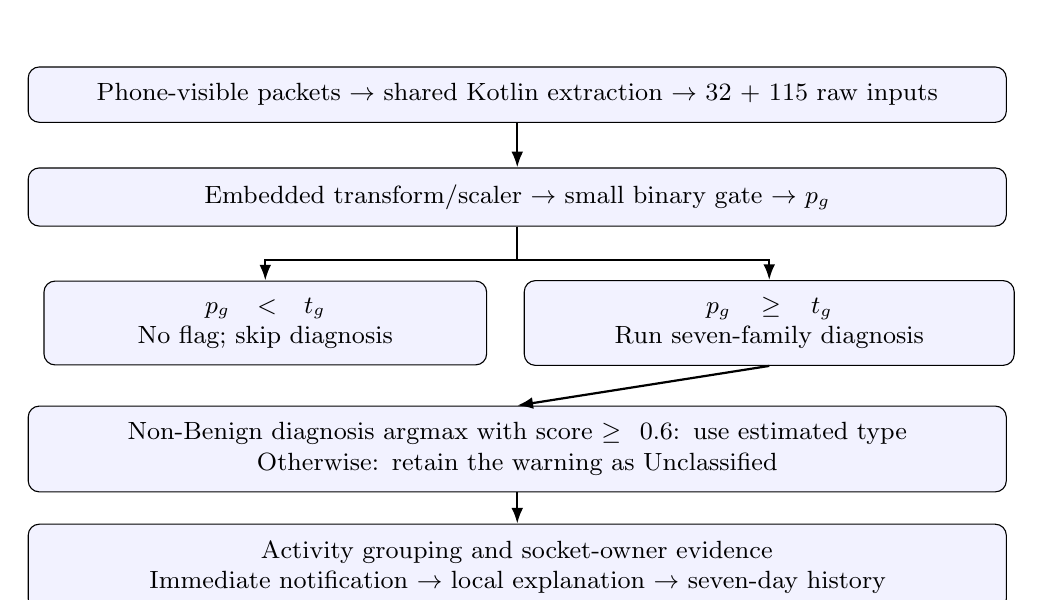
\begin{tikzpicture}[node distance=7mm]
\node[box,text width=12cm] (x) at (0,0) {Phone-visible packets $\rightarrow$ shared Kotlin extraction $\rightarrow$ 32 + 115 raw inputs};
\node[box,text width=12cm] (g) at (0,-1.3) {Embedded transform/scaler $\rightarrow$ small binary gate $\rightarrow$ $p_g$};
\node[box,text width=5.2cm] (quiet) at (-3.2,-2.9) {$p_g<t_g$\\No flag; skip diagnosis};
\node[box,text width=5.8cm] (diag) at (3.2,-2.9) {$p_g\geq t_g$\\Run seven-family diagnosis};
\node[box,text width=12cm] (type) at (0,-4.5) {Non-Benign diagnosis argmax with score $\geq0.6$: use estimated type\\Otherwise: retain the warning as Unclassified};
\node[box,text width=12cm] (end) at (0,-6.0) {Activity grouping and socket-owner evidence\\Immediate notification $\rightarrow$ local explanation $\rightarrow$ seven-day history};
\draw[arr] (x)--(g);\draw[arr] (g.south)--(0,-2.1)-|(quiet.north);\draw[arr] (g.south)--(0,-2.1)-|(diag.north);
\draw[arr] (diag.south)--(type.north);\draw[arr] (type.south)--(end.north);
\end{tikzpicture}
\end{center}
\important{In v2, diagnosis never cancels a positive binary gate. Benign, weak or unavailable diagnosis becomes Unclassified while retaining the warning. This differs from the earlier v6 cascade, where the second stage could eliminate all positives.}

\section{Offline results, with exact support}

{\small
\begin{longtable}{@{}p{0.57\textwidth}r@{}}
\toprule
Selected full-pipeline metric & Value\\\midrule\endhead
Typed accuracy & 99.8782\%\\
Typed macro F1 & 94.0323\%\\
Binary precision / recall & 99.5415 / 99.6424\%\\
Benign false flags / total & 729 / 940,095\\
Missed attack-labeled views & 568\\
Gate threshold / type threshold & 0.7858333333 / 0.6\\
\bottomrule\end{longtable}
}


{\small
\begin{longtable}{@{}lrrrrr@{}}
\toprule
Class & Support & Typed P & Typed R & Typed F1 & Gate recall\\\midrule\endhead
Benign & 940,095 & 99.940 & 99.922 & 99.931 & --\\
Bot & 640 & 54.286 & 92.031 & 68.290 & 92.188\\
Brute Force & 2,442 & 99.959 & 99.672 & 99.815 & 99.672\\
DDoS & 17,840 & 99.627 & 97.220 & 98.408 & 97.343\\
DoS & 90,084 & 99.932 & 99.960 & 99.946 & 99.967\\
Port Scan & 47,688 & 99.971 & 99.996 & 99.983 & 99.998\\
Web Attack & 140 & 95.385 & 88.571 & 91.852 & 96.429\\
\bottomrule\end{longtable}
}

The selected complete pipeline had typed accuracy 99.8782\%, macro F1 94.0323\%, binary precision 99.5415\%, binary recall 99.6424\% and benign FPR 0.07755\%: 729 false flags among 940,095 benign views. It missed 568 of 158,834 attack-labeled views. These are grouped raw-capture benchmark measurements, not live phone accuracy.

\section{Why performance dropped relative to the context benchmark}
The historical context comparison used 848,349 CSV rows and 110 inputs; v2 used 1,098,929 re-extracted test views, 147 inputs, different history visibility/windows, different class proportions, a new architecture, weighted losses and a new decision policy. A headline difference between these cohorts cannot isolate the effect of ``alignment.''

The main diagnosed weaknesses were:
\begin{itemize}
\item \textbf{Bot/Benign ambiguity:} final Bot typing included 589 true Bot views and 496 benign views, producing only 54.29\% precision. Strong confidence did not make these false Bot assignments correct. Reset-like benign inputs overlapped attack patterns; rare-class weighting can influence the tradeoff but was not proved the sole cause.
\item \textbf{Gate bottleneck for DDoS:} the gate rejected 474 of 17,840 DDoS views before diagnosis. Of those, 418 would have been correctly typed by a counterfactual standalone diagnosis. Lowering the gate globally could increase benign warnings.
\item \textbf{Web subtype scarcity:} correct Web-family recall was 102/104 HTTP-brute-force views, 21/34 XSS and 1/2 SQL views. Two SQL examples cannot establish reliability.
\item \textbf{Limited visible semantics:} only 2/34 XSS test views had the script-like indicator; 20/34 had gap/truncation observations and 14/34 lacked a parsed HTTP request. The parser reads only bounded first-header evidence, not unlimited bodies or encrypted content.
\item \textbf{Selection and overfitting tradeoffs:} a later diagnosis checkpoint could improve recall while reducing precision. More epochs or a larger model was not a demonstrated universal repair.
\end{itemize}
Shared-campaign/host dependence remains. Exact 147-input matches to training occurred for 28,730 test views (2.6144\%), even with zero connection-group overlap. A train-only scaler refit matched within about $1.2\times10^{-9}$ mean and $1.7\times10^{-9}$ scale error, so the audit did not identify test-fitted normalization as the cause of these failures.

\section{Executed v2 dry runs}

{\small
\begin{longtable}{@{}lrrrrr@{}}
\toprule
Reference label & Old row & Gate score & Route? & Diagnosis max & Final v2\\\midrule\endhead
Benign & 0 & 0.000000 & No & Benign* & Benign\\
Bot & 684012 & 0.999959 & Yes & Bot & Bot\\
DDoS & 825582 & 0.001237 & No & DDoS* & Benign\\
Web Attack & 522766 & 0.999944 & Yes & Web Attack & Web Attack\\
\bottomrule\end{longtable}
}
An asterisk marks a counterfactual diagnosis computed for analysis even though the live gate would skip it.
For the deterministic DDoS example in the table, the gate probability is about 0.001237, so v2 returns Benign and does not invoke diagnosis. For explanatory analysis only, we also ran diagnosis on that vector: its DDoS score is about 0.875191. This illustrates a gate bottleneck using actual frozen weights; this counterfactual extra inference is not performed on a gate-negative event by the live app.

For the first aligned Web-labeled example, the gate is about 0.999944 and diagnosis Web score about 0.999967, producing a Web Attack warning. This successful old-benchmark example does not contradict the later misses on different phone requests.

\chapter{Stage 5: repair v3, measured and rejected}
\section{What remained fixed and what changed}
Before repair, we preserved a rollback snapshot/tag and v2 inference bundle. Repair reused exactly the v2 rows, raw feature contract, grouping, normalization and model dimensions. It introduced no new attack labels or manual phone cases. The experiment measured loss/sampling, calibration, routing and full-pipeline selection.

Three treatments, three seeds and both models produced 18 jobs and 720 completed epochs. All used the same architecture, per-seed initial state, AdamW settings, batch size 512, 40-epoch/update budget and no early stopping. The treatments were:
\begin{enumerate}
\item \textbf{Unweighted:} natural-frequency unweighted loss with seeded full-cohort shuffling.
\item \textbf{Moderate weights:} relative class weights capped at three times the Benign weight.
\item \textbf{Difficult-benign sampling:} unweighted loss, with 10\% of epoch draws from a training-only pool of 54,695 difficult Benign rows and 90\% from the full cohort. Total updates match, but row exposure intentionally differs.
\end{enumerate}
Original v2 weights and an unchanged-weights routing/calibration-only control were also reported. The same total epochs do not mean identical example frequencies when a sampling treatment intentionally changes them.

\section{Calibration and two-threshold routing}
Split the existing validation set into disjoint connection groups: 547,200 calibration rows and 641,524 selection rows, seed 9301. Fit a positive shared logit scale and biases using natural-frequency calibration negative log-likelihood. Freeze these parameters before evaluating the policy grid. Neither calibration nor policy fitting uses the final test.

The selected repair used unweighted gate seed 2 epoch 40 and diagnosis seed 2 epoch 39. Its calibrated gate scale is approximately 0.739892 with bias $-0.550573$. Diagnosis uses a shared scale approximately 0.762645 and seven fitted class biases. These transformations adjust scores; they do not provide new packet evidence.

The selected routing policy has low threshold 0.1, high threshold 0.99, review acceptance 0.5 and type confidence 0.5:
\begin{itemize}
\item Below 0.1: no diagnosis and no warning.
\item From 0.1 to below 0.99: diagnosis reviews the event; warn only when $1-p_{\mathrm{Benign}}\geq0.5$.
\item At or above 0.99: warn regardless of diagnosis; use Unclassified if naming is weak.
\end{itemize}
A review is not automatically an alert. High warnings cannot be vetoed. The final v2 pipeline does not use these repair thresholds.

Joint selection used predeclared checkpoint shortlists: top validation-ranked gate epochs plus final, and diagnosis epochs ranked through composed-pipeline behavior with additional Bot/Web and final candidates. All saved epochs remain available, but this was not an exhaustive search of every possible gate/diagnosis epoch pair. Calibration and policy comparison used validation groups, with no final-test winner replacement.

\section{Matched comparison and the decision}
Both pipelines were scored on the same already-opened 1,098,929 test views. This is a stronger matched comparison than comparing the old CSV benchmark to raw-packet v2, but it is still development evidence rather than a new blind test.

{\small
\begin{longtable}{@{}lrr@{}}
\toprule
Matched metric & V2 & Repair\\\midrule\endhead
Binary precision & 99.54150 & 99.81043\\
Binary recall & 99.64239 & 99.77650\\
Binary F1 & 99.59192 & 99.79346\\
Benign FPR & 0.07755 & 0.03202\\
Typed macro F1 & 94.0323 & 94.0076\\
Benign flags & 729 & 301\\
Attack misses & 568 & 355\\
\bottomrule\end{longtable}
}


{\small
\begin{longtable}{@{}lrr@{}}
\toprule
Class & Preserved v2 $P/R/F_1$ & Selected repair $P/R/F_1$\\\midrule\endhead
Benign & 99.94 / 99.92 / 99.93 & 99.96 / 99.97 / 99.97\\
Bot & 54.29 / 92.03 / 68.29 & 79.75 / 60.94 / 69.09\\
Brute Force & 99.96 / 99.67 / 99.82 & 99.92 / 99.67 / 99.79\\
DDoS & 99.63 / 97.22 / 98.41 & 99.42 / 99.54 / 99.48\\
DoS & 99.93 / 99.96 / 99.95 & 99.92 / 100.00 / 99.96\\
Port Scan & 99.97 / 100.00 / 99.98 & 99.97 / 100.00 / 99.98\\
Web Attack & 95.38 / 88.57 / 91.85 & 91.79 / 87.86 / 89.78\\
\bottomrule\end{longtable}
}

Benign flags fell from 729 to 301, a 58.71\% reduction. Aggregate binary recall improved slightly because the larger DDoS/DoS classes improved. However, Bot binary detection fell from 590/640 to 391/640; exact Bot recall fell from 92.031\% to 60.938\%. Web binary detection fell from 135/140 to 124/140. Macro F1 fell slightly from 94.0323\% to 94.0076\%.

The protocol required at least 0.5 pp macro-F1 improvement and 5 pp Bot-precision improvement; no benign-FPR increase; no more than 0.1 pp aggregate binary-recall loss, 1 pp per-class binary-recall loss, 2 pp typed-recall loss or 1 pp typed-precision loss. Both selection and test comparisons had to pass. The selected repair failed. We retained v2 as the user-requested fallback. This was not a declaration that v2 was production ready; it prevented adopting a repair that hid important losses behind an aggregate improvement.

All nine treatment/seed finalists and the routing-only control appear in Appendix D. We did not choose a new winner by sorting their final test results. A candidate that looks better after opening the test is a diagnostic lead for a future prospective experiment.

\section{Repair dry run}
On the first old aligned Bot-labeled example, calibrated repair gate probability is about 0.674625. It enters the review band, diagnosis gives Bot about 0.99999994, and a Bot warning is retained. On the first aligned DDoS example, its gate is only about 0.001872, so no diagnosis is invoked and it is missed. Individual examples can succeed or fail even when a class's aggregate recall rises or falls; they do not replace the classwise table.

\chapter{What runs on the phone}
\section{Capture and feature processing}
The tested phone is an ARM64 Pixel 6a. Its recorded device-contract inventory reported Android 17, API 37, ABI \code{arm64-v8a}. This is the tested device environment, distinct from the app's compile/target SDK 34 and PARROT's emulator environment. Live capture requires an already-rooted owned device and a compatible Android tcpdump executable. The app uses a foreground monitoring service and a persistent Android notification. USB/ADB is used for installation, control and evidence collection; it is not the classifier input.

The capture command uses \code{tcpdump --immediate-mode -i any -U -s 768 -w -}. Packets are copied into the local monitor; the app is not implemented as a VPN and does not route every packet through an external server. A 768-byte capture limit is not an assertion that the model reads all application data. The IP/transport parser and bounded 512-byte payload-prefix logic determine what numeric evidence is available.

The app parses packets, maintains ordered flow state and 5/30/300-second histories, emits eligible snapshots, runs the gate and conditionally diagnosis, attaches attribution, stores/updates an activity and posts a notification. A flow may close on a reset immediately or after a timeout/FIN boundary. Detection latency therefore includes collection/flow closure as well as model execution.

An initial experimental v2 build, \code{0.12.1} / code 35, revealed a live delivery-clock bug before attack testing: the collector advanced using wall time while delayed capture packets were still arriving, rejecting 10,034 of 35,833 observed packets as late at that snapshot. The code-36 service/clock correction retained the trained feature definitions and weights and added delivery-clock regression checks. This is distinct from the later DatasetLab replay start-boundary issue. The later clean test counters should not be retroactively assigned to that failed build.

One fixed implementation is used for both training extraction and the Android contract. The native checks include rapid-history updates, phone-only visibility, zero-duration handling, HTTP reassembly/duplicate handling, SQL negative controls, encrypted scope, expiry and the non-vetoing gate policy. A delivery-clock regression check ensures backlog processing is not confused with packet event time. Earlier implementation/timing issues were recorded and corrected before the validated v2 deployment.

\section{Model export and device verification}
ExecuTorch PTE file sizes are 82,820 bytes for the gate and 949,788 bytes for diagnosis, together about 0.985\,MiB. Normalization is embedded. Manifests pin input contract and model hashes; startup self-checks compare known numerical outputs. Small model size does not include the Android runtime, buffers, APK or optional Llama.

On 960 reference rows, work-PC native export checks had zero binary/final-type decision flips. Maximum native/reference errors were 0.0001220703125 for gate and 0.001953125 for diagnosis. On the phone, 14 self-check rows had zero pipeline flips. A passive capture replay compared 204 rows, 29,988 feature values, with maximum feature error zero. These tests establish execution/feature agreement within their scope, not attack accuracy.

V2 was installed on 20 November 2026 at approximately 17:46 IST as \code{0.12.2-aligned-v2-test}, code 36. The gate is \code{gate_s0}; diagnosis is \code{diagnosis64_s1}. Earlier export reports marked native verification pending when first created; the later device deployment records supersede that historical pending state. The subsequent controlled tests used these same frozen model hashes.

\section{App attribution}
The UID resolver snapshots connected sockets and matches both directions of protocol/address/port pairs. Recent matches are retained for about ten seconds. An unambiguous UID can be mapped through Android's package manager to an app package/label. Shared UIDs, short-lived sockets, unmatched connections and OS responses can remain unknown.

For an incoming attack, the identified app is typically the \emph{recipient socket owner}, not the attacker. A closed-port scan may be answered by the operating system without an application socket. The app must not claim that an unknown package launched the attack, or blame a receiving app merely because it owned the target socket.

\section{Activities, notifications and seven-day history}
Flagged observations are grouped into related activities using a fingerprint and a recent aggregation interval. One activity can be revised as more flow flags arrive. SQLite stores observations, explanations and user feedback with seven-day retention, subject to pruning. The interface supports reviewing/filtering history and expected/suspicious/unsure feedback; that feedback is recorded as unverified user judgment, not an automatic training label.

A flag count measures model decisions. An activity count measures grouped records. A notification snapshot counts currently visible notifications, which may have been grouped, updated or dismissed. A successful explanation is another separate state. Thus 500 scan flow flags and four activity notifications are compatible.

\section{Local Llama and warm model caching}
The explanation model is Llama 3.2 1B Instruct in SpinQuant INT4 EO8 form. Its PTE is 1,135,951,488 bytes (about 1.06\,GiB), with a 2,183,982-byte tokenizer. These optional weights are much larger than the two classifiers and are downloaded separately under their upstream license.

After a flag, the app constructs structured evidence: estimated family, gate/type scores, timing, counts, endpoint/direction information, best-effort ownership and history/parser limitations. Llama is asked for a short factual explanation, generally at most 65 words, with an appropriate manual check. It is not sent the attack's expected test label or asked to determine ground truth.

Generation runs in an isolated \code{:llama} process with one active task and a persistent queue. Detection notifications do not wait for the language model. A generation timeout is about 90 seconds. Drafts are checked against the supplied facts; unavailable, malformed or unsupported output uses deterministic evidence guidance. Dismissal/cancellation and memory pressure can release the worker.

Warm caching retains loaded weights for approximately 120 seconds of idle time while monitoring continues. Each request resets prompt context. This saves repeated loading without carrying one activity's conversation into another. It does not mean seven days of raw packets or all past prompts are kept in Llama memory.

One early technical explanation test accepted local Llama prose in about 26 seconds including verification/loading, with sampled peak PSS around 1.27 million KiB. That is one measured run, not a latency guarantee or battery benchmark. In the later v2 scan/load campaign, explanations completed through \emph{evidence fallback}; they must not be reported as accepted Llama-generated summaries.

\section{One complete live-case walkthrough}
For a closed-port probe, a PC sends SYN and the phone replies with RST/ACK. As an illustrative two-packet calculation, if the response follows 10\,ms later, duration is 10,000 microseconds, forward/backward counts are 1/1, payload bytes can be 0/0, SYN count 1, RST count 1 and ACK count 1. Payload-byte rate is zero and packet rate is 200/s. This calculation illustrates extraction only; no model output is invented for this hand-made example.

The collector appends the relevant prior-history and protocol values to make 147 inputs. The frozen raw-input wrappers transform/standardize them, the gate returns a score, and positive events enter diagnosis. On the recorded fast-scan episode, this chain produced actual Port Scan and Unclassified flags, which became four grouped activities. The explanation identified a possible scan, retained uncertain ownership where appropriate and supplied a manual check. That observed episode is the live evidence; the arithmetic example simply explains how packet observations become features.

\chapter{Actual controlled phone testing}
\section{The experiment setup}
TrafficLab is a separate disposable Android target app. The PC sends actual TCP/HTTP requests over the private LAN. The target contains dummy accounts, an intentionally injectable in-memory database, isolated JavaScript execution and a two-slot test resource. Only the configured controller is admitted; the session and request budgets are bounded. NIDS observes traffic independently.

For verified cases, compare three evidence sources: the controller's actual connection/request outcomes; target-side login/effect/resource events; and packet/native feature/decision traces. Match complete connection identities and timestamps, not merely a shared time window. Labels are never assigned by reading the classifier's prediction.

Warm the current history for 340 seconds, observe each case for 130 seconds, and isolate independent cases by at least 305 seconds after the last relevant traffic/decision. The user originally launched individual commands manually; later they explicitly authorized the remaining automated sequence. No model/threshold was changed to force a test alert.

\section{What each profile actually did}
\begin{longtable}{p{0.21\textwidth}p{0.72\textwidth}}
\toprule Profile & Mechanism and independently observed effect\\\midrule\endhead
Benign & Eight ordinary HTTP requests per control. Used before/after the campaign to check quiet behavior on a small control.\\
PortScan & Attempt connections to one open lab port and 128 verified closed ports. A TCP scan need not generate an HTTP event. Retransmissions/segmentation can produce more decisions than connection attempts.\\
SlowScan & Probe one open plus 31 closed ports with slower spacing, testing longer-history sensitivity.\\
PasswordGuessing & Submit 32 guesses to the dummy HTTP account, 31 failing and one succeeding. This belongs to the dataset's Web family, not FTP/SSH-Patator.\\
SQLInjection & Submit one ordinary search and two injections. The target confirms that the dummy database returned an otherwise unavailable test record.\\
XSS & Submit a script to the isolated vulnerable page. A harmless marker confirms script execution. It exposes neither phone files nor an operating-system shell.\\
Connection exhaustion & Occupy both dummy resource slots for about five seconds and submit 16 requests. Two hold slots and 14 are refused, showing limited target-service resource denial.\\
HTTPFlood & Send 128 bounded requests with at most eight workers. All received HTTP 200; a burst alone does not demonstrate service denial or distributed origins.\\
Beacon & Trigger 12 intended phone-to-PC PING/PONG connections, roughly three seconds apart, representing periodic communication. The actual attempts timed out.\\
\bottomrule
\end{longtable}

\section{Frozen v2 results}
\begin{longtable}{p{0.18\textwidth}p{0.37\textwidth}r r p{0.19\textwidth}}
\toprule Case & Verified traffic/effect & Flags & Notices & Interpretation\\\midrule\endhead
Normal controls & 8 before + 8 after ordinary requests & 0 & 0 & Quiet small controls.\\
Fast scan & 129 ports; 128 closed & 500 & 4 & 476 Scan, 24 unknown; all 128 closed connections flagged at least once.\\
HTTP guessing & 31 failed + 1 valid login & 0 & 0 & Guessing episode missed.\\
SQL injection & 2 confirmed injections + 1 control & 0 & 0 & Both missed after exact traffic correlation.\\
XSS & 1 confirmed isolated execution & 0 & 0 & Missed.\\
Resource denial & 2 held slots, 14 denied requests & 0 & 0 & Bounded service-denial case missed.\\
HTTP burst & 128 HTTP 200 responses & 71 & 3 & 1 DoS, 70 unknown; denial not established.\\
Slow scan & 32 ports; 31 closed & 110 & 3 & 105 Scan, 5 unknown; 29/31 closed connections flagged.\\
Beacon/retry & Each run: 12 timeouts, no exchange & 0 & 0 & Inconclusive connectivity case.\\
\bottomrule
\end{longtable}
Flags are matched flow segments, not independent attacks. Visible notices are saved related-notification snapshots. No per-class population recall or false-alerts/day estimate can be calculated from this small correlated matrix alone.

Fast-scan exact typing covered 126 of 128 closed-port connections at least once. Slow-scan exact typing covered 28 of 31, while binary flags covered 29 of 31. A connection flagged multiple times contributes one connection to those coverage counts, but multiple rows to the flow-flag counts.

\section{The SQL result that initially looked positive}
The terminal initially showed two model flags and one activity during the SQL test's time window, and a flag was seen on the phone. Detailed source-port/start-time/packet correlation found all three SQL test connections were predicted Benign. The two flags came from unrelated loopback traffic. Both injections had a SQL-like input indicator, so the miss could not simply be blamed on the text never reaching the parser.

Their gate scores were approximately 0.064063 and $9.78\times10^{-28}$, below 0.785833. Standalone diagnosis replay also predicted Benign. Thus the correct test outcome is \emph{two confirmed SQL effects missed}, not ``SQL injection detected.'' The repeated paste of the same terminal output was counted once.

\section{Other verified misses and their interpretation}
For the XSS case, a script-like indicator was present and target execution was confirmed, but the gate logit was about $-104.2933$, giving a near-zero score. Standalone diagnosis was also Benign. For the resource-denial case, all 16 segments were Benign and the largest gate score was only about 0.003616. Merely bypassing the gate would not automatically fix these examples.

The actual phone features can be valid, finite and exactly reproducible while still being outside the learned positive distribution. An audit found observed authentication-failure inputs in 394 original Benign training views and zero original attack-class training views. That is evidence of a positive-supervision gap, not a proof that this one feature explains every failure.

\section{Why Beacon was inconclusive}
Both the original attempt and the permitted retry emitted phone-to-PC connection attempts without a completed PING/PONG exchange. Read-only firewall inspection found an enforced inbound TCP block matching the PC receiver executable. The narrow temporary allow rule did not override it. The temporary rule was removed by its cleanup process; existing blocks remained unchanged.

A failed communication path does not supply a Bot-positive label or a model-recall estimate. A future test needs a reachable controller under approved network configuration. We did not disable managed policy or count the timeouts as successful bot communication.

\section{What these tests establish}
They demonstrate working capture, inference, scan-related warnings, grouping and notifications on the owned Pixel. Clean saved counters and independent packet/native checks reduce the chance that the observed misses are only log/capture failures. They also demonstrate important Web and resource-denial misses. Sixteen quiet normal requests cannot establish low long-duration false positives, and a bounded HTTP burst cannot establish broad DoS/DDoS coverage.

\chapter{Stage 6: building a real phone dataset extension}
\section{Why we collected new data}
The user proposed supplementing the large existing dataset with actual controlled phone traffic in exactly the deployed feature format, rather than inventing synthetic attack vectors. This addresses an important gap: a model can have millions of desktop/lab views and very few verified examples matching the phone's Web/authentication observations.

We built DatasetLab 0.1.0 as a separate target. It adds session-specific dummy credentials, per-connection IDs, request/response/effect logs and varied positive/normal actions. The installed NIDS v2, feature implementation and thresholds remain fixed during collection. DatasetLab's source is separate from the detector, so the expected label cannot silently become a classifier input.

\section{Positive actions and matched normal controls}
Positives are verified HTTP password guessing, HTTP password spraying, SQL injection and XSS. Spraying means trying one wrong password across several dummy accounts; it remains a fine subtype of Web Attack. SQL and XSS require actual isolated effect confirmation. Credential attack labels describe verified controlled attempts, not necessarily successful account compromise.

Controls include successful login, an ordinary incorrect password, normal HTTP, varied-size pages, code-like search text, ordinary server errors and legitimate bursts. A single failed login or a string resembling code can be benign. Matching these controls prevents a model from being rewarded simply for treating all errors or script-looking text as attacks.

The target uses invented data, isolated rendering, an exact controller restriction and bounded lifetime/connection budget. It does not send ground-truth headers to the detector. Unrelated phone background traffic is kept unknown; it is not blanket-labeled Benign.

\section{Capture procedure and quality gates}
The older manual-test companion recordings were filtered to test ports and captured only 96 bytes/packet. They were useful packet evidence, but could not reconstruct complete phone-wide history and payload indicators. They were not silently reused as a complete retraining dataset.

New collection records phone-local \code{any}-interface PCAP with snaplen 768 and a 100,000-record limit, including the full relevant background context. It warms history for 340 seconds and allows a final flush. Bulk PCAP transfer happens after capture, avoiding a wireless-ADB streamed-capture feedback loop. Transfers are hash checked.

Acceptance requires container integrity, no premature cap/stop, zero kernel drops, healthy native queues, exact per-connection packet accounting, independent controller/target identity agreement and all eligible 147-value native/replay inputs matching within $10^{-4}$. Unconfirmed effects or ambiguous mapping reject the intended example/session instead of inventing a label. Rejected/interrupted evidence is retained.

\section{The segmentation-boundary problem found by the pilot}
The first pilot quality check failed: the auxiliary PCAP began before the native app stream. Persistent TCP connections then had different 30-second segmentation phases in offline replay. More warm-up alone would not necessarily align those segment boundaries.

The replay adapter was made deterministic using the earliest native-observed TCP/UDP flow-start boundary. This uses stream timing, not labels, scores or the size of a model error. We did not relax the feature tolerance or alter the feature contract to force parity. The original rejection remains preserved.

The accepted development pilot contained 56 requests: 24 normal and 32 Web attempts/effects, with 8,232 feature values compared and maximum error zero. It is excluded from research fitting and final evaluation. Target and negative-label smoke checks also verified actual effects and rejection of mismatched socket proofs. Small technical training/export/evaluation smokes checked the automation; their scores are not research accuracy.

\section{Frozen sessions, labels and exact counts}
Twenty chronological sessions were assigned in advance: 14 training (10 mixed, 4 benign-only), 3 validation (2 mixed, 1 benign-only) and 3 test (2 mixed, 1 benign-only). Held-out SQL/XSS forms and timing ranges were specified. Keep whole sessions and their contexts together. This is same-phone/same-app session generalization, not an unseen-device/day/site study.

All 20 sessions passed quality gates. They contain 1,216 unique controlled labeled segments: 768 normal and 448 Web Attack. The split counts and subtypes are:

{\small
\begin{longtable}{@{}lrrrr@{}}
\toprule
Unique controlled subtype & Train & Val. & Test & Total\\\midrule\endhead
http password guessing & 120 & 24 & 24 & 168\\
http password spraying & 80 & 16 & 16 & 112\\
sql injection & 60 & 12 & 12 & 84\\
xss & 60 & 12 & 12 & 84\\
normal http & 56 & 12 & 12 & 80\\
successful login & 56 & 12 & 12 & 80\\
ordinary failed login & 56 & 12 & 12 & 80\\
normal search or code & 56 & 12 & 12 & 80\\
normal page & 56 & 12 & 12 & 80\\
ordinary server error & 56 & 12 & 12 & 80\\
legitimate http burst & 192 & 48 & 48 & 288\\
\textbf{Unique total} & 848 & 184 & 184 & 1,216\\
\bottomrule\end{longtable}
}

The 11 earlier diagnostic recordings, old phone test matrix, all software smokes and the development pilot are excluded from the actual new fitting/final test. No Bot/FTP/SSH/DoS/DDoS positives are claimed from this collection.

\section{Combining old and new training data}
Original train/validation/test memberships are preserved. Add only new training-session rows to training. Repeat those 848 real training rows eight times in the training cache so their contribution is not overwhelmed by almost five million old rows. This is declared exact resampling, not 6,784 independent observations or fabricated traffic. Validation/test phone rows are added once.


{\small
\begin{longtable}{@{}lrrrr@{}}
\toprule
Partition & Original rows & Unique new & Replay factor & Combined rows\\\midrule\endhead
Train & 4,956,674 & 848 & 8 & 4,963,458\\
Validation & 1,188,724 & 184 & 1 & 1,188,908\\
Test & 1,098,929 & 184 & 1 & 1,099,113\\
\bottomrule\end{longtable}
}

Refit normalization using the combined training rows only. Original raw validation/test examples and memberships remain fixed, but their \emph{standardized numerical values} change consistently when the new training-fitted scaler changes. We do not claim that adding new data leaves every normalized old tensor identical.

Frequency-derived class weights also recompute from the augmented training labels. The weighting rule is unchanged; its numerical weights need not equal the original v2 values after the class counts change.

The architecture, loss/training loop, learning rate, batch size, seed set and 40-epoch budget match v2. The extra rows increase updates from 9,682 to 9,695 per epoch: 13 extra updates/epoch, 520 over 40 epochs per job. Thus the same epoch count is not exactly the same optimizer-update count in this augmentation experiment.

\section{Current training status and final comparison plan}
At the evidence cutoff, \textbf{5 of six jobs were complete}; the remaining jobs were active or queued. The report does not publish partial candidate accuracy as a final result. All six jobs train for 40 epochs without early stopping, at most two concurrently, saving every epoch and best/last/final states.

The planned evaluation compares complete gate-plus-diagnosis candidates on validation, freezes selected weights/policy before final test access and reports original and new-phone cohorts separately. It includes classwise precision/recall/F1/support, binary FPR/recall, subtypes, per-session behavior and unknown types. New phone held-out scores were not inspected for this report's dry runs. Old frozen examples were used instead.

Passing collection parity proves that the input format and independent labels agree; it does not prove the trained update will improve recall or preserve old-class performance. No automatic deployment follows training. Candidate hashes, native parity, ordinary-use controls and prospective live tests remain necessary before replacement.

\chapter{Reproducibility, engineering checks and research claims}
\section{Recorded environment}
The work took place on the user's work PC using Windows PowerShell 5.1 and local Ubuntu/WSL for training. The measured Python training environment records Python 3.12.14, PyTorch 2.14.1 with CUDA 13.0, NumPy 2.2.6, pandas 3.0.6, scikit-learn 1.9.1 and an NVIDIA RTX 2000 Ada GPU. The context extractor also requires Numba 0.68.1 and llvmlite 0.50.0. Package versions are recorded observations, not requirements to install whatever is newest later.

The Android source pins compile/target SDK 34, minimum API 26, Android Gradle Plugin 8.7.3, Kotlin 2.0.21 and the Gradle 9.6.0 wrapper. Java 21 was used for the verified build. Python export tooling uses ExecuTorch 1.5.0; the Android runtime dependency is ExecuTorch Android 1.5.1. These are distinct components and should not be described as one identical version string. Native parity checks address numerical compatibility within the tested scope.

\section{What the smoke tests mean}
Software smokes used tiny generated fixtures or explicitly designated development rows. They checked parsing, shapes/gradients, pruning masks, checkpoint/resume, evaluation, export and label guards. They reduce automation risk. They do not supply research training examples, verified phone attacks or deployment accuracy.

For the submission, validation included four dataset-free model/label checks; fresh CPU paper/context smokes; a tiny aligned train/evaluate/TorchScript/ExecuTorch smoke; Kotlin feature/policy/clock checks; all current Android module/instrumentation builds; Windows setup/preview checks; direct child-script launch; source/link/private-file checks; and a clean Git-checkout contract test.

The first hosted GitHub run exposed a missing explicit Numba dependency hidden by the existing local environment and a failure in an Android SDK replacement action. We pinned Numba/llvmlite and used the verified preinstalled SDK on Ubuntu 24.04. The corrected hosted run \code{44821013266} passed both the Python contracts/paper/context smokes and Android assembly. A later documentation-only commit recorded that evidence. These checks confirm build/automation behavior, not scientific generalization.

\section{Persistence, power loss and version history}
Long-running jobs were launched through persistent local schedulers, with progress/status/log files and duplicate-run locks. Closing the chat or reaching a chat limit does not itself stop those processes. A PC shutdown, sleep, WSL termination or hardware failure can interrupt them. After the reported power interruption, the repair workflow resumed from retained state rather than starting a new unrecorded experiment.

Epoch checkpoints include optimizer and random-generator state as required by each workflow. Completed jobs are skipped; interrupted jobs resume from their last complete checkpoint, potentially repeating an unfinished epoch. Best-validation, best-training where applicable, final and last serve different purposes. No early stopping removed the opportunity to complete the declared epoch budgets.

Rollback snapshots preserved earlier model bundles before repair/deployment. The current gate and diagnosis hashes are recorded in Appendix F. No report-building operation changes a model, threshold, training split or running training source. Temporary file-access/session issues discussed in the conversation were operational interruptions; conclusions here are anchored to saved artifacts rather than assuming that an inaccessible file implied failed training. No definitive universal root cause is invented for every historical access issue.

\section{GitHub submission and what is excluded}
The user supplied \url{https://github.com/vishwajeet-singh-bhati/Android-nids} and authorized terminal publication under their account. We prepared an isolated current-source snapshot with readable directories for Android, four paper-to-current experiment stages, validation tools, models, results and documentation. A clean source root was used instead of pushing the entire older workstation history. The latest publication before this report was \code{e0100ed}; this report's documentation commit can be newer.

The source snapshot contains the current small inference models and a pinned optional Llama download manifest, not the large language-model weights. Research datasets, raw phone recordings, app histories, credentials, old packet fixtures, unused legacy weights, caches and epoch checkpoint dumps are excluded. No ZIP was created; the user deferred that until the end.

Public benchmark runs can be regenerated after obtaining the matching publisher files and following the documented layout/configurations. Exact private-phone-cohort retraining cannot be independently reproduced from source alone while those recordings are excluded. Another researcher can repeat the collection method but will obtain a different timed cohort. Historical repair and pre-paper evidence remains locally preserved; the curated repository does not imply that every historical experiment's full source/data bundle is included.

\section{What could support an incremental paper?}
\textbf{Model selection at the cutoff:} context-pruned-30 has the best score on the historical CSV benchmark. That benchmark contains dependent laboratory history and does not justify deploying it as the best phone detector. V2 is the installed experimental pipeline with shared phone-visible inputs. The matched repair was rejected for class regressions, and the phone-data candidates have no final accepted comparison yet. There is no validated general-purpose production winner at this cutoff.

The plausible research story is a carefully documented progression: transparent TSANet reconstruction; matched context/control experiment; demonstration of benchmark-to-phone failure; a shared phone-visible feature implementation; independently labeled real-phone collection; and prospective comparison of the repaired data pipeline. Negative findings and failed repairs are valuable evidence when their protocols and limits are explicit.

Adding context, increasing model size or attaching Llama alone does not establish novelty. No exhaustive related-work review or first-of-its-kind claim is made here. The current evidence also cannot support a state-of-the-art mobile detection claim. Stronger publication evidence would require independent later campaigns/devices, matched ablations, multiple seeds, uncertainty at the independent-episode/group level, representative normal-use hours, measured detection delays/resources and class/subtype coverage.

The methodology was informed by CIC-IDS2017 provenance and the cautions on sampling, leakage, shortcuts and evaluation in Arp et al.'s USENIX Security 2022 work. These are methodological references, not a claim of certification. The benchmark audit, limited new-phone cohort and open-test development history must remain visible in any paper.

\chapter{What remains to test and what our setup can prove}
\section{Coverage by class}
\begin{longtable}{p{0.17\textwidth}p{0.35\textwidth}p{0.41\textwidth}}
\toprule Family & Completed phone evidence & Remaining coverage work\\\midrule\endhead
Benign & Small HTTP controls, plus independently labeled new normal actions. & Long normal-use sessions, legitimate multi-client bursts, different apps/devices/networks and false alerts per observation hour.\\
Port Scan & Fast and slower scans detected by fixed v2. & Independent repetitions, different port sets/rates and discovery/retry controls; assess episode recall/delay.\\
Web Attack & Confirmed SQL/XSS/HTTP-guessing examples missed; new varied real data collected. & Finish candidate evaluation and repeat prospective tests; encrypted semantics remain unavailable.\\
Brute Force & Existing dummy HTTP login belongs to Web, not the FTP/SSH family. & Actual disposable FTP and SSH services on the phone, dummy credentials and authentication logs; normal failed-login controls.\\
DoS & Bounded two-slot denial missed; ordinary HTTP burst flagged with weak typing. & Several controlled request/slow-connection patterns and measured impact on normal requests; distinguish target pressure from sender/Wi-Fi bottlenecks.\\
DDoS & No completed distributed phone experiment. & Multiple independent clients, verified origins and measured service impact under a fixed bounded protocol.\\
Bot & Intended Beacon connections timed out. & Reachable approved local controller and harmless agent with verified check-in/dummy-command/reply behavior. This cannot certify detection of every malware family.\\
\bottomrule
\end{longtable}

\section{The proposed extra-PC arrangement}
The user offered SSH access to two or three additional PCs and confirmed that they share the phone's local network. This is a proposed setup; hosts/credentials were not supplied and no such remote test was run. The main work PC can coordinate, collect results and send low-rate normal probes. Two additional physical PCs can originate bounded concurrent traffic. A third can provide another source or independent normal probe.

SSH is the control channel; test traffic should travel from each selected PC directly to the phone's isolated service. Verify the actual source addresses in phone captures. Current TrafficLab accepts only one controller, so its target restrictions must be extended to a fixed explicit set of test sources before this campaign. Merely opening many workers on one existing client does not provide the same evidence as independent source machines.

A two-source experiment is a useful starting design, not a universal source count that proves complete DDoS coverage. A shared access point/router and small target impose scale/bottleneck limits. Confirm whether the test service actually slows or refuses ordinary requests, record the measured impact, and separate that from capture loss or network failure. Larger source count by itself is not a correctness metric.

An alternative discussed was two Linux VMs on the existing PC, whose approximately 64\,GB RAM makes small VMs plausible. Their routing/unique visible identities were not configured or verified. VMs share physical resources; results would need to be reported as a virtualized multi-source experiment. Extra physical PCs avoid that particular shared-host limitation but still require connectivity checks.

\section{Internet, device access and visibility limits}
The classifiers and installed Llama operate locally. The controlled PC-to-phone tests need a working private LAN, not public internet. USB debugging/ADB remains useful for installation, test control and evidence retrieval. Initial dependency/model downloads and genuine online-app evaluation can require internet separately.

Training after completed collection does not require the phone to remain connected. Actual capture, installation and on-device tests do. A successful APK installation does not prove root/SELinux/tcpdump compatibility or a working capture stream on another phone.

No network detector can directly inspect plaintext hidden by encryption unless the system supplies an authorized decryption mechanism; this implementation does not. Purely local file/process behavior without observable network evidence is outside this detector's current input. Traffic exclusively between other machines is outside the watched-phone feature scope.

\section{How future test outcomes should be recorded}
Use a fixed candidate and thresholds, check packet/input health, record target ground truth independently and reserve prospective test sessions. Report each case as correctly typed detection, detection with wrong/unknown type, miss, or inconclusive delivery/ground-truth failure. Pair every suspicious pattern with suitable ordinary traffic and use episode-level as well as flow-level reporting.

When a case exposes a weakness, preserve the result. Once it informs a repair, it is development material. A later retest can verify the repair on that case, but a genuinely independent accuracy claim needs newly reserved evidence. This rule is why the report keeps the original context audit, repair regressions, SQL correlation correction and inconclusive Beacon visible.

\appendix
\chapter{Exact 32-feature flow layout}
The following is the fixed selected order, numbered from one. In Python, subtract one for zero-based indices. The publisher-CSV and phone-re-extracted measurements share names/units where intended, but their segmentation/visibility definitions differ as explained in Chapters 5--6.

{\small
\begin{longtable}{@{}rp{0.48\textwidth}p{0.30\textwidth}@{}}
\toprule
Position & Feature & Meaning / unit\\\midrule\endhead
1 & Flow Duration & Microseconds\\
2 & Total Fwd Packets & Count\\
3 & Total Backward Packets & Count\\
4 & Total Length of Fwd Packets & Payload bytes\\
5 & Total Length of Bwd Packets & Payload bytes\\
6 & Fwd Packet Length Max & Payload bytes\\
7 & Fwd Packet Length Min & Payload bytes\\
8 & Fwd Packet Length Mean & Payload bytes\\
9 & Fwd Packet Length Std & Payload bytes\\
10 & Bwd Packet Length Max & Payload bytes\\
11 & Bwd Packet Length Min & Payload bytes\\
12 & Bwd Packet Length Mean & Payload bytes\\
13 & Bwd Packet Length Std & Payload bytes\\
14 & Flow Bytes/s & Payload bytes/second\\
15 & Flow Packets/s & Packets/second\\
16 & Flow IAT Mean & Microseconds\\
17 & Flow IAT Std & Microseconds\\
18 & Flow IAT Max & Microseconds\\
19 & Flow IAT Min & Microseconds\\
20 & Fwd IAT Total & Microseconds\\
21 & Fwd IAT Mean & Microseconds\\
22 & Fwd IAT Std & Microseconds\\
23 & Fwd IAT Max & Microseconds\\
24 & Fwd IAT Min & Microseconds\\
25 & Bwd IAT Total & Microseconds\\
26 & Bwd IAT Mean & Microseconds\\
27 & Bwd IAT Std & Microseconds\\
28 & Bwd IAT Max & Microseconds\\
29 & Bwd IAT Min & Microseconds\\
30 & SYN Flag Count & Count\\
31 & RST Flag Count & Count\\
32 & ACK Flag Count & Count\\
\bottomrule\end{longtable}
}

For the phone implementation, sample standard deviations use zero for fewer than two observations. Missing direction totals/minima/means are encoded as defined finite zeros. Undefined rates for zero duration are zero. These are contract choices, not evidence that a genuinely unobserved application field is known to be zero.

\chapter{Exact history and auxiliary layouts}
\section{Historical 78-value context}
For each window in order 120, 300, 900 seconds: source role, then destination role, then the 13 statistics below. With the 32 flow values preceding context, the source/destination ranges are 33--45/46--58, 59--71/72--84, and 85--97/98--110.
\begin{enumerate}
\item Log1p prior completed-flow occurrences.
\item Log1p outgoing packets.
\item Log1p incoming packets.
\item Log1p outgoing payload bytes.
\item Log1p incoming payload bytes.
\item Log1p distinct peers.
\item Log1p distinct remote ports.
\item Log1p distinct local ports.
\item Fraction with no peer-direction packets.
\item Fraction with reset present.
\item Fraction with SYN present.
\item Fraction TCP.
\item Fraction UDP.
\end{enumerate}
Identifiers are used only for grouping/counting. The trained context branch receives standardized numbers. Empty history has the declared numeric zeros before scaling.

\section{Current 115-value context and 147 combined positions}
Replace the window sequence with 5, 30, 300 seconds. For each role, use the same first 13 statistic types, followed by log1p observed authentication failures, HTTP requests and Web indicators. This yields 16 statistics per role/window.
\begin{center}\begin{tabular}{lll}\toprule Combined positions & Meaning & Count\\\midrule
1--32 & Flow statistics & 32\\
33--48 / 49--64 & 5-second source / destination & 16 + 16\\
65--80 / 81--96 & 30-second source / destination & 16 + 16\\
97--112 / 113--128 & 300-second source / destination & 16 + 16\\
129--146 & Current-flow auxiliary fields & 18\\
147 & Logarithmic capped history age & 1\\\bottomrule\end{tabular}\end{center}


{\small
\begin{longtable}{@{}rp{0.72\textwidth}@{}}
\toprule
Combined position & Flow auxiliary observation\\\midrule\endhead
129 & http requests\\
130 & http responses\\
131 & http auth failures\\
132 & http 4xx\\
133 & http 5xx\\
134 & login-like requests\\
135 & SQL-like requests\\
136 & script-like requests\\
137 & TLS prefix seen\\
138 & cleartext HTTP seen\\
139 & payload packets\\
140 & duplicate payload fragments\\
141 & header buffer full\\
142 & payload gaps or truncation\\
143 & basic auth seen\\
144 & long header seen\\
145 & SSH banner seen\\
146 & FTP banner or credentials seen\\
\bottomrule\end{longtable}
}

Position 147 is $\log(1+\min(300,\text{history age in seconds}))$, reaching $\log(301)\approx5.707110$ at full age. First-header evidence and numeric lexical indicators are intentionally limited. Seeing a SQL-like or script-like string is neither necessary nor sufficient for proving an attack.

\chapter{Complete software fixture and executed dry runs}
\section{A full input that can be written out without distributing a dataset}
The report collector also built one hand-constructed software fixture and actually ran it through the frozen models. It is never used for training, selection or accuracy. It represents a two-packet SYN then RST/ACK observation 10\,ms apart, with two prior similar conversations involving one peer and two target ports in each history horizon. There is no assigned Benign/attack truth. Actual live-case results remain in Chapter 9.

The complete flow input, in Appendix A order, is:
\begin{lstlisting}
flow = [10000, 1, 1, 0, 0, 0, 0, 0, 0, 0, 0, 0, 0,
        0, 200, 10000, 0, 10000, 10000,
        0, 0, 0, 0, 0, 0, 0, 0, 0, 0, 1, 1, 1]
L2, L3 = log(2), log(3)
source13 = [L3,L3,L3,0,0,L2,L3,L2,0,1,1,1,0]
destination13 = [L3,L3,L3,0,0,L2,L2,L3,0,1,1,1,0]
historical_context78 = (source13 + destination13) * 3
current_context115 = ((source13 + [0,0,0]) +
                      (destination13 + [0,0,0])) * 3
current_context115 += [0] * 18 + [log(301)]
\end{lstlisting}
The list multiplication means three repeated window blocks, not numerical multiplication of every value by three. Source/destination use reversed local/remote port counts. There are no HTTP or payload observations in this fixture. Historical and current pipelines apply their own fitted preprocessing; this exercise is a dataflow walkthrough, not a matched scientific comparison of their traffic semantics.


{\small
\begin{longtable}{@{}p{0.29\textwidth}lrr@{}}
\toprule
Frozen model/pipeline & Output & Largest diagnosis score & Gate score\\\midrule\endhead
baseline & Benign & 0.997888 & --\\
pruned\_30 & Benign & 0.999965 & --\\
pruned\_40 & Benign & 0.999949 & --\\
control\_baseline & Benign & 0.808990 & --\\
control\_pruned\_30 & Benign & 0.955349 & --\\
context\_baseline & Benign & 1.000000 & --\\
context\_pruned\_30 & Benign & 1.000000 & --\\
Aligned v2 & Benign & 0.994170 & 0.029194\\
Selected repair & Benign & 0.820366 & 0.000251\\
\bottomrule\end{longtable}
}

For every multiclass row, the largest output probability determines the displayed class. For v2 and repair, the route/alert policy is applied before using diagnosis. Any diagnosis computed counterfactually for explanation is explicitly marked; a negative live gate would skip it.

\section{Probabilities on deterministic old-cohort examples}
The following probabilities are computed on CPU from actual saved weights. Display rounding can make a very small number look zero or a score look exactly one. They are model scores, not certainty. The full machine-readable evidence records more digits and source-file hashes.
\subsection{historical CSV test -- Benign example, row 1}
First five raw flow values: \code{60921, 1, 1, 40, 94}.

{\small
\begin{longtable}{@{}p{0.26\textwidth}rrrrrrr@{}}
\toprule
Model [final output] & B & Bot & BF & DDoS & DoS & Scan & Web\\\midrule\endhead
baseline [Benign] & 1.000000 & 0.000000 & 0.000000 & 0.000000 & 0.000000 & 0.000000 & 0.000000\\
pruned\_30 [Benign] & 1.000000 & 0.000000 & 0.000000 & 0.000000 & 0.000000 & 0.000000 & 0.000000\\
pruned\_40 [Benign] & 1.000000 & 0.000000 & 0.000000 & 0.000000 & 0.000000 & 0.000000 & 0.000000\\
control\_baseline [Benign] & 0.999999 & 0.000000 & 0.000000 & 0.000000 & 0.000000 & 0.000000 & 0.000000\\
control\_pruned\_30 [Benign] & 1.000000 & 0.000000 & 0.000000 & 0.000000 & 0.000000 & 0.000000 & 0.000000\\
context\_baseline [Benign] & 1.000000 & 0.000000 & 0.000000 & 0.000000 & 0.000000 & 0.000000 & 0.000000\\
context\_pruned\_30 [Benign] & 1.000000 & 0.000000 & 0.000000 & 0.000000 & 0.000000 & 0.000000 & 0.000000\\
\bottomrule\end{longtable}
}

\subsection{historical CSV test -- Bot example, row 343}
First five raw flow values: \code{105130, 4, 3, 206, 134}.

{\small
\begin{longtable}{@{}p{0.26\textwidth}rrrrrrr@{}}
\toprule
Model [final output] & B & Bot & BF & DDoS & DoS & Scan & Web\\\midrule\endhead
baseline [Bot] & 0.046869 & 0.946322 & 0.000001 & 0.000000 & 0.000147 & 0.006662 & 0.000000\\
pruned\_30 [Bot] & 0.000155 & 0.999830 & 0.000000 & 0.000000 & 0.000002 & 0.000012 & 0.000000\\
pruned\_40 [Bot] & 0.001599 & 0.998339 & 0.000000 & 0.000000 & 0.000001 & 0.000062 & 0.000000\\
control\_baseline [Bot] & 0.020950 & 0.973814 & 0.000001 & 0.000000 & 0.000000 & 0.005236 & 0.000000\\
control\_pruned\_30 [Bot] & 0.004901 & 0.994537 & 0.000000 & 0.000000 & 0.000000 & 0.000562 & 0.000000\\
context\_baseline [Bot] & 0.000000 & 1.000000 & 0.000000 & 0.000000 & 0.000000 & 0.000000 & 0.000000\\
context\_pruned\_30 [Bot] & 0.000000 & 1.000000 & 0.000000 & 0.000000 & 0.000000 & 0.000000 & 0.000000\\
\bottomrule\end{longtable}
}

\subsection{historical CSV test -- Web Attack example, row 2168}
First five raw flow values: \code{5.72206e+06, 3, 1, 0, 0}.

{\small
\begin{longtable}{@{}p{0.26\textwidth}rrrrrrr@{}}
\toprule
Model [final output] & B & Bot & BF & DDoS & DoS & Scan & Web\\\midrule\endhead
baseline [Benign] & 0.826422 & 0.000239 & 0.000291 & 0.000172 & 0.000702 & 0.001079 & 0.171095\\
pruned\_30 [Benign] & 0.788683 & 0.000023 & 0.000088 & 0.000025 & 0.000541 & 0.000928 & 0.209713\\
pruned\_40 [Benign] & 0.827870 & 0.000035 & 0.000471 & 0.000058 & 0.000421 & 0.000494 & 0.170651\\
control\_baseline [Benign] & 0.839119 & 0.000052 & 0.000324 & 0.000007 & 0.001062 & 0.000219 & 0.159218\\
control\_pruned\_30 [Benign] & 0.854824 & 0.000000 & 0.000004 & 0.000003 & 0.000420 & 0.000100 & 0.144649\\
context\_baseline [Web Attack] & 0.000000 & 0.000000 & 0.000000 & 0.000000 & 0.000000 & 0.000000 & 1.000000\\
context\_pruned\_30 [Web Attack] & 0.000000 & 0.000000 & 0.000000 & 0.000000 & 0.000000 & 0.000000 & 1.000000\\
\bottomrule\end{longtable}
}

\subsection{opened aligned v2 test -- Benign example, row 0}
First five raw flow values: \code{1240.97, 10, 9, 3104, 3036}.
Diagnosis rows below include counterfactual analysis when routing is false; live routing is stated in the main walkthrough.

{\small
\begin{longtable}{@{}p{0.26\textwidth}rrrrrrr@{}}
\toprule
Model [final output] & B & Bot & BF & DDoS & DoS & Scan & Web\\\midrule\endhead
v2 [Benign] & 1.000000 & 0.000000 & 0.000000 & 0.000000 & 0.000000 & 0.000000 & 0.000000\\
repair [Benign] & 1.000000 & 0.000000 & 0.000000 & 0.000000 & 0.000000 & 0.000000 & 0.000000\\
\bottomrule\end{longtable}
}

\subsection{opened aligned v2 test -- Bot example, row 684012}
First five raw flow values: \code{65578, 5, 4, 1858, 128}.
Diagnosis rows below include counterfactual analysis when routing is false; live routing is stated in the main walkthrough.

{\small
\begin{longtable}{@{}p{0.26\textwidth}rrrrrrr@{}}
\toprule
Model [final output] & B & Bot & BF & DDoS & DoS & Scan & Web\\\midrule\endhead
v2 [Bot] & 0.000914 & 0.999086 & 0.000000 & 0.000000 & 0.000000 & 0.000000 & 0.000000\\
repair [Bot] & 0.000000 & 1.000000 & 0.000000 & 0.000000 & 0.000000 & 0.000000 & 0.000000\\
\bottomrule\end{longtable}
}

\subsection{opened aligned v2 test -- DDoS example, row 825582}
First five raw flow values: \code{1.71128e+06, 8, 6, 20, 11595}.
Diagnosis rows below include counterfactual analysis when routing is false; live routing is stated in the main walkthrough.

{\small
\begin{longtable}{@{}p{0.26\textwidth}rrrrrrr@{}}
\toprule
Model [final output] & B & Bot & BF & DDoS & DoS & Scan & Web\\\midrule\endhead
v2 [Benign] & 0.124755 & 0.000002 & 0.000000 & 0.875191 & 0.000025 & 0.000027 & 0.000000\\
repair [Benign] & 0.759141 & 0.000032 & 0.000000 & 0.239559 & 0.000000 & 0.001268 & 0.000000\\
\bottomrule\end{longtable}
}

\subsection{opened aligned v2 test -- Web Attack example, row 522766}
First five raw flow values: \code{5.38272e+06, 4, 2, 0, 0}.
Diagnosis rows below include counterfactual analysis when routing is false; live routing is stated in the main walkthrough.

{\small
\begin{longtable}{@{}p{0.26\textwidth}rrrrrrr@{}}
\toprule
Model [final output] & B & Bot & BF & DDoS & DoS & Scan & Web\\\midrule\endhead
v2 [Web Attack] & 0.000033 & 0.000000 & 0.000000 & 0.000000 & 0.000000 & 0.000000 & 0.999967\\
repair [Web Attack] & 0.015650 & 0.000000 & 0.000000 & 0.000001 & 0.000000 & 0.000005 & 0.984344\\
\bottomrule\end{longtable}
}


\chapter{All declared aligned and repair finalists}
\section{Aligned v2: best-validation and final checkpoints}
Values below are percentages. For standalone diagnosis rows, attack detection is derived from that component's declared attack score; it is not the same as the final selected gate-plus-diagnosis pipeline. Thus a component row must not be substituted for the deployed cascade's result. All entries are old opened benchmark evidence.

{\small
\begin{longtable}{@{}p{0.32\textwidth}rrrr@{}}
\toprule
Component: checkpoint & Attack P & Attack R & Benign FPR & Typed macro F1\\\midrule\endhead
gate\_s0:best & 99.541 & 99.642 & 0.0775 & --\\
gate\_s0:final & 99.546 & 99.861 & 0.0770 & --\\
diagnosis64\_s0:best & 99.396 & 99.889 & 0.1025 & 93.554\\
diagnosis64\_s0:final & 99.448 & 99.906 & 0.0937 & 92.352\\
gate\_s1:best & 99.484 & 99.863 & 0.0874 & --\\
gate\_s1:final & 99.423 & 99.876 & 0.0980 & --\\
diagnosis64\_s1:best & 98.334 & 99.993 & 0.2862 & 93.485\\
diagnosis64\_s1:final & 99.538 & 99.778 & 0.0783 & 93.534\\
gate\_s2:best & 99.493 & 99.794 & 0.0858 & --\\
gate\_s2:final & 99.046 & 99.951 & 0.1626 & --\\
diagnosis64\_s2:best & 99.192 & 99.960 & 0.1375 & 93.585\\
diagnosis64\_s2:final & 99.414 & 99.861 & 0.0995 & 86.738\\
aligned32\_s0:best & 99.036 & 99.970 & 0.1645 & 93.300\\
aligned32\_s0:final & 99.496 & 99.889 & 0.0854 & 92.549\\
wire\_only32\_s0:best & 79.864 & 99.542 & 4.2402 & 87.770\\
wire\_only32\_s0:final & 79.765 & 99.503 & 4.2648 & 87.421\\
\bottomrule\end{longtable}
}


\section{Repair: complete treatment/seed finalists}
The table retains every frozen per-treatment/seed finalist plus the unchanged-weights routing control. These are matched opened-test results. The selected repair was unweighted seed 2 by the prescribed validation procedure, and still failed the better/fallback rule. We did not promote whichever row happens to look most attractive on this test.

{\small
\begin{longtable}{@{}lrrrrrr@{}}
\toprule
Treatment & Seed & FP & FN & Attack P & Attack R & Macro F1\\\midrule\endhead
unweighted & 0 & 659 & 215 & 99.586 & 99.865 & 94.052\\
unweighted & 1 & 651 & 282 & 99.591 & 99.822 & 93.111\\
unweighted & 2 & 301 & 355 & 99.810 & 99.776 & 94.008\\
moderate & 0 & 507 & 280 & 99.681 & 99.824 & 93.809\\
moderate & 1 & 641 & 262 & 99.597 & 99.835 & 93.320\\
moderate & 2 & 565 & 351 & 99.645 & 99.779 & 93.914\\
hard\_benign & 0 & 767 & 415 & 99.518 & 99.739 & 93.332\\
hard\_benign & 1 & 232 & 457 & 99.854 & 99.712 & 93.581\\
hard\_benign & 2 & 619 & 296 & 99.611 & 99.814 & 93.343\\
routing\_only & 0 & 256 & 431 & 99.839 & 99.729 & 93.752\\
\bottomrule\end{longtable}
}


\chapter{Historical appendix: work before the paper restart}
\section{Why this appendix is separate}
Earlier chat discussed AndMal, RC4, three v5 approaches and a v6 binary/diagnosis design. These are preserved as historical context, not silently presented as versions of the TSANet paper experiment. Their feature contracts, datasets and labels differ. The curated submission starts at the paper reconstruction and contains one current application version, not all older binaries.

\section{Earliest AndMal packet-window task}
The early model's unit was a 32-packet window with 12 metadata channels and 128 payload bytes per packet, trained for benign versus malicious-associated Android capture labels. The locally recorded family-holdout split had 577,806 training, 124,374 validation and 125,045 test windows; app/capture/family grouping was recorded and split leakage-error checks were empty. These counts do not imply attack-specific SQL/Bot/DDoS labels. The later CIC seven-family task is fundamentally different.

The alternate group-random split had 578,636/124,219/124,370 windows. Split strategy changes which families are seen and cannot be mixed into one accuracy claim. Source captures were capped during that processing. These local inventory figures explain the user's earlier question about AndMal2017 versus the current dataset; AndMal and AAGM are not interchangeable names.

\section{RC4's two detectors}
RC4 used a short-flow detector with first-eight-packet metadata $[8,9]$, a mask and 16 context values, and a separate 27-value endpoint-behavior detector. The recorded parameter counts were 24,721 and 62,657. The behavior detector required consecutive confirmation; the short-flow path emitted unconfirmed pattern evidence. It was not the current 147-input TSANet cascade.

On the later opened v5 evaluation, the preserved RC4 short-flow control detected Bot 139/226 (61.5\%), scan 9,023/9,064 (99.5\%) and DDoS 10,772/11,405 (94.4\%). It flagged 854/58,144 CIC benign units, 0/64 PARROT captures and 4/39 AAGM captures. RC4 behavior raw scan recall was 100\% but confirmed recall was 42.9\%; raw/confirmed DDoS recall was 94.7\%/94.2\%. These are distinct correlated-unit/capture measures, not population phone accuracy.

\section{The three v5 approaches}
Approach A trained a larger general binary detector. Approach B used a shared representation with separate label heads: Bot/scan/DDoS for short-flow and scan/DDoS for behavior. Approach C trained a metadata teacher from scratch, then distilled a smaller student using hard labels plus temperature-2 teacher targets. It was not ET-BERT/YaTC fine-tuning.

Both tasks used variants general/specialist/teacher/student across seeds 0, 1 and 2, giving 24 jobs at 40 epochs each with all 960 epoch checkpoints retained. Up to three workers overlapped. Short-flow sampling used 240,000 examples/epoch; behavior used 120,000. Those epochs are sampled update budgets, not full passes over their respective 1,543,183-prefix and 692,593-bucket corpora. Training-only hard-negative mining and balanced sampling were recorded.

The short-flow encoder maps nine packet channels into a temporal convolutional representation, applies residual depthwise/pointwise temporal blocks, masked pooling, a 16-value context branch and fusion. The behavior encoder is a residual MLP over 27 values. General/specialist width/depth are 192/4, teacher 512/8, student 96/3. Specialist heads share the encoder; union thresholds were calibrated jointly. Model sizes were:
\begin{center}\begin{tabular}{lrr}\toprule Variant & Short-flow parameters & Behavior parameters\\\midrule
General & 993,217 & 618,049\\
Specialist & 1,030,467 & 636,674\\
Teacher & 11,198,977 & 8,556,033\\
Student & 214,849 & 119,617\\\bottomrule\end{tabular}\end{center}

The preselected short-flow specialist seed 1 had Bot 76.1\%, scan 99.8\% and DDoS 99.3\% raw recall, but 1,138/58,144 CIC benign units, 6/64 PARROT captures and 1/39 AAGM captures flagged. The preferred behavior general seed 2 had raw scan 97.1\% but confirmed scan 41.4\%, and raw/confirmed DDoS 90.6\%/90.1\%. It flagged 17/73,755 CIC benign buckets and 1/39 AAGM captures. No candidate passed all frozen gates.


{\small
\begin{longtable}{@{}p{0.31\textwidth}rrrrrr@{}}
\toprule
Old candidate & Params & Epoch & Recall & CIC FP & PARROT & AAGM\\\midrule\endhead
shortflow\_teacher\_s0 & 11,198,977 & 22 & 70.84 & 107/58144 & 0/64 & 0/39\\
behavior\_teacher\_s0 & 8,556,033 & 5 & 89.88 & 14/73755 & 0/64 & 0/39\\
shortflow\_general\_s0 & 993,217 & 22 & 48.11 & 2/58144 & 0/64 & 0/39\\
behavior\_general\_s0 & 618,049 & 16 & 92.15 & 14/73755 & 0/64 & 0/39\\
shortflow\_specialist\_s0 & 1,030,467 & 17 & 99.17 & 1611/58144 & 6/64 & 1/39\\
behavior\_specialist\_s0 & 636,674 & 20 & 89.26 & 4/73755 & 0/64 & 0/39\\
shortflow\_student\_s0 & 214,849 & 20 & 69.10 & 108/58144 & 0/64 & 0/39\\
behavior\_student\_s0 & 119,617 & 4 & 92.15 & 11/73755 & 0/64 & 0/39\\
shortflow\_teacher\_s1 & 11,198,977 & 12 & 59.65 & 31/58144 & 1/64 & 0/39\\
behavior\_teacher\_s1 & 8,556,033 & 2 & 94.63 & 23/73755 & 0/64 & 0/39\\
shortflow\_general\_s1 & 993,217 & 17 & 72.44 & 111/58144 & 0/64 & 0/39\\
behavior\_general\_s1 & 618,049 & 2 & 91.74 & 19/73755 & 0/64 & 3/39\\
shortflow\_specialist\_s1 & 1,030,467 & 28 & 99.23 & 1138/58144 & 6/64 & 1/39\\
behavior\_specialist\_s1 & 636,674 & 13 & 93.39 & 7/73755 & 3/64 & 0/39\\
shortflow\_student\_s1 & 214,849 & 38 & 64.95 & 54/58144 & 0/64 & 0/39\\
behavior\_student\_s1 & 119,617 & 7 & 93.60 & 16/73755 & 0/64 & 0/39\\
shortflow\_teacher\_s2 & 11,198,977 & 23 & 69.42 & 101/58144 & 0/64 & 0/39\\
behavior\_teacher\_s2 & 8,556,033 & 2 & 54.55 & 18/73755 & 0/64 & 0/39\\
shortflow\_general\_s2 & 993,217 & 13 & 73.02 & 121/58144 & 0/64 & 1/39\\
behavior\_general\_s2 & 618,049 & 1 & 91.53 & 17/73755 & 0/64 & 1/39\\
shortflow\_specialist\_s2 & 1,030,467 & 23 & 99.05 & 1816/58144 & 3/64 & 1/39\\
behavior\_specialist\_s2 & 636,674 & 17 & 44.42 & 4/73755 & 3/64 & 0/39\\
shortflow\_student\_s2 & 214,849 & 37 & 69.78 & 114/58144 & 0/64 & 0/39\\
behavior\_student\_s2 & 119,617 & 5 & 90.08 & 14/73755 & 0/64 & 0/39\\
\bottomrule\end{longtable}
}

Candidates were installed one at a time for bounded high-port phone probes. Both profiles captured all 104 generated SYN attempts. V5 short-flow detected 5/8 slow, 10/12 moderate and 24/24 rapid scan attempts as warnings, while also flagging 3/8 slow single-port retries. Its paired RC4 short-flow control flagged 33/40 bounded burst attempts. These probe shapes were not verified malware or DoS labels. RC4 was restored after those experiments; neither v5 candidate earned production promotion.

\section{Recorded illustrative dry runs for the older variants}
The earlier architecture-walkthrough artifact ran one invented parsed-metadata example through real frozen weights without sending packets. At the full eight-packet prefix, the RC4 short-flow logit was $-19.773787$ versus threshold $2.194104$, producing no warning. V5 seed-0 general, teacher and student logits were $-25.120564$, $-31.169973$ and $-23.109875$, respectively, each below its own threshold. Specialist seed 0 returned three logits $[-32.951229,-40.293274,-47.070202]$, all below their respective thresholds.

For the paired behavior example, RC4 second-101 logit was $-9.969679$ versus $-3.284726$ threshold; the following second also stayed below threshold, so no consecutive confirmation occurred. V5 behavior seed-0 general, teacher and student logits were $-10.815851$, $-11.245574$ and $-11.011199$, also negative relative to their thresholds. These are software traces, not evidence that ordinary phone use or attacks are always classified correctly.

\section{The earlier v6 cascade and why it failed}
V6 used a 72-value aggregate binary gate (width 64 or 96) and a larger diagnosis model (width 192 or 256) with 12-channel packet sequences, masks and 72-value context. The gate had residual MLP blocks; diagnosis used six residual temporal convolution blocks with dilations 1/2/4 repeated, masked pooling, a context MLP, fusion and ten historical output categories. This is not the seven-class v2 design.

All 12 jobs completed 40 epochs, retaining 480 epoch checkpoints. The preselected width-64 seed-0 gate plus width-192 seed-1 diagnosis had gate recall 57.85\%, but the final cascade detected 0/2,083 held-out positives because its second-stage cutoff rejected them. It flagged 2/245,549 benign windows and detected 0/1,019 development Bot windows. Numerical export and 1,211 Android feature snapshots passed parity, illustrating again that implementation agreement is not detection success.

Coverage was also deficient: training had 1,483,947 benign windows but only 99 scan, 195 DoS, 2,017 credential-associated, 10 Web, 1,485 Bot, 780 infiltration and 1,674 Heartbleed windows; DDoS and mixed-suspicious had zero training windows. The preflight had not enforced required positive-class coverage. Held-out positives covered only DoS, credential-associated and infiltration-associated cases. A model cannot be claimed validated on absent classes.

A post-hoc pair reached 95.92\% held-out binary recall but only 41.90\% Bot development recall and roughly 94.6\% unknown types among flagged holdout windows. It did not meet the intended general detection plus reliable diagnosis goal. V6 was not deployed. This failure motivated stronger class-coverage preflights, independent end-to-end policy checks and the later v2 rule that diagnosis cannot veto a positive high-confidence gate.

\chapter{Evidence index, reproduction and model identity}
\section{Primary saved records}
Paths below are relative to the local project root unless marked public. Older repair/pre-paper evidence is locally retained and is not all part of the curated current-source repository.
\begin{longtable}{p{0.29\textwidth}p{0.64\textwidth}}
\toprule Topic & Primary record\\\midrule\endhead
Paper assumptions & \code{experiments/tsanet_paper/PROTOCOL.md}\\
Paper metrics/counts & \code{validation/reports/tsanet_paper/baseline_results.json} and \code{classwise.csv}\\
Context comparison & \code{validation/reports/tsanet_context/comparison.json} and \code{VALIDATION.md}\\
Leakage/dependence audit & \code{validation/reports/publication_validity_audit/AUDIT.md} and numeric companions\\
Aligned data/decisions & \code{validation/reports/phone_alignment_v2/data_report.json}, \code{evaluation.json}, \code{DROP_ANALYSIS.md}\\
Repair comparison & \code{validation/reports/phone_repair_v3/evaluation.json}, \code{selection.json}, \code{CLASSWISE_COMPARISON.md}\\
Native deployment & \code{validation/reports/v2_phone_deployment/device_native.json}, \code{native_offline.json}, \code{deployment.json}\\
Actual phone cases & \code{validation/reports/v2_automated_phone_tests/RESULTS.md}; exact case reviews under \code{validation/reports/manual_phone_tests/}\\
New collection/QC & \code{experiments/phone_capture_v1/DATASHEET.md}; \code{validation/reports/phone_capture_v1/collection_summary.json}\\
Augmentation counts & \code{validation/reports/phone_capture_training_v1/data_report.json}\\
Dataset comparison & \code{validation/reports/dataset_comparison/provenance.json}\\
Older v5/v6 & \code{validation/reports/robust_v5_audit/}, \code{robust_v5_phone/}, \code{cascade_v6/}\\
Report numerical trace & \code{docs/project_report/REPORT_EVIDENCE.json}; read-only collector \code{tools/report/collect_report_evidence.py}\\
Public guides/results & Repository \code{docs/}, \code{results/}, \code{models/current/MODEL_CARD.md}, \code{reproducibility/VALIDATION.json}\\
\bottomrule
\end{longtable}

\section{Frozen current inference hashes}
\begin{lstlisting}
gate PTE SHA-256:
99e5f3b62b1f6940cd2fb40d05c2edb14b3a7fb83c3bc1f989e63879202ca529
diagnosis PTE SHA-256:
585f43e8bf4299f755036e9ccbe55121fce14d8ff59a67fcfdcfb4ba8af951dd
feature-contract SHA-256:
0a6f7c956c3fe8cc8329395c62098eefd735d9f49b82176ebcce42c7f609993c
\end{lstlisting}
The report collector hashes its aggregate source records and executes frozen old-model dry runs on CPU. It never trains, changes thresholds, connects to a phone or scores the new held-out phone cohort. Static report examples and old opened-cohort inspection cannot replace future prospective evaluation.

\section{Public reproduction entry points}
After obtaining datasets and setting up the documented environment, run from the curated repository root:
\begin{lstlisting}
python reproduce.py doctor
python -m pytest tests -q
python reproduce.py paper --smoke
python reproduce.py context --smoke
python reproduce.py paper
python reproduce.py context
python reproduce.py aligned prepare
python reproduce.py aligned train
python reproduce.py aligned export
\end{lstlisting}
Paper/context training uses Linux/WSL. Export requires the separate pinned export dependencies. The full aligned pipeline requires raw captures and substantial storage/compute; a smoke fixture does not replace those inputs. Build/install, rooted-device prerequisites and optional Llama download steps are documented in the repository's Android setup guide.

The controlled test commands use \code{python reproduce.py phone test --profile PROFILE}, where PROFILE is one of Benign, PortScan, SlowScan, PasswordGuessing, SQLInjection, XSS, ConnectionExhaustion, HTTPFlood or Beacon. A \code{--preview} produces no traffic. These existing profiles do not automatically implement the proposed new multi-PC, FTP/SSH or completed bot-controller tests.

For the existing local running campaign, PowerShell status/log commands are:
\begin{lstlisting}
.\validation\Run-PhoneCapture.ps1 -Action Status
Get-Content .\runs\phone_capture_training_v1\scheduler_status.json
Get-Content .\runs\phone_capture_training_v1\logs\diagnosis_s2.log -Tail 30 -Wait
\end{lstlisting}
Stopping log viewing does not stop detached training. Use the documented campaign controls for an intentional stop/resume; do not silently edit frozen training code during execution.

\section{Overleaf compilation}
Upload only \code{Android_NIDS_Project_Report.tex} into a blank Overleaf project, set it as the main document, select pdfLaTeX and compile. Recompile for the contents/page references if required. All tables and TikZ figures are embedded. The optional companion evidence JSON is for audit and is not a compilation input. No private captures, copyrighted paper PDF, external image downloads, bibliography tool or ZIP is required.

\begin{thebibliography}{9}
\bibitem{tsanet} J. Malode et al., \emph{A Lightweight Embedded Intelligent Threat Detection System Using TSANet on Android Platforms}, ISED 2025. \url{https://doi.org/10.1109/ISED67359.2025.11404952}. The supplied paper informed the reconstruction; undisclosed implementation details are listed explicitly in Chapter 3.
\bibitem{cic} Canadian Institute for Cybersecurity, \emph{CIC-IDS2017 dataset}. \url{https://www.unb.ca/cic/datasets/ids-2017.html}.
\bibitem{aagm} Canadian Institute for Cybersecurity, \emph{Android Adware and General Malware dataset}. \url{https://www.unb.ca/cic/datasets/android-adware.html}.
\bibitem{parrot} PARROT dataset publisher record. \url{https://zenodo.org/records/16368932}. Local inventory and accepted/excluded files are recorded separately.
\bibitem{arp} D. Arp et al., \emph{Dos and Don'ts of Machine Learning in Computer Security}, USENIX Security 2022. \url{https://www.usenix.org/conference/usenixsecurity22/presentation/arp}.
\bibitem{repo} Project source and current reproducibility documentation. \url{https://github.com/vishwajeet-singh-bhati/Android-nids}.
\end{thebibliography}
\end{document}
